%% ceci est un commentaire 
%% il faut toujours commencer par \documentclass[type de papier, taille de texte]{sytle du document}
\documentclass[a4paper,10pt]{report} %%%% sytle du document : report/book/article


%%%%%%%%%%%%%%%%%%%%%%%%%%%%%%%%%%%%%%%%%%%%%%%%%%%%%%%%%%%%%%%%%%%%%%%%%%%%%%%
%% la suite est une collection des "package" ou des "librararies" pour utiliser des codes spécifiques

%% il vous suffit de les copie-coller quand vous créez un nouveau document TeX (ou bien en ajouter plus si besoin).
\usepackage[utf8]{inputenc} %% pour les accents en français
\usepackage[frenchb]{babel} %% pour un format français
\usepackage{graphicx} %% pour afficher des graphiques
\usepackage{amsmath} %% pour écrire des symboles (maths), des équations, etc.
\usepackage{amssymb}
\usepackage{color}
\usepackage{bm} %% pour lister des citations/la biblio
\usepackage{hyperref} %% pour inserer des liens internet
\usepackage{cleveref} %% pour faire des références uax équations, tableaux, etc.
\usepackage{cite}
\usepackage{float}
%\usepackage{setspace} %% pour changer l'espace entre les lignes
%\linespread{1.6} %% pour changer l'espace entre les lignes



%%%%%%%%%%%%%%%%%%%%%%%%%%%%%%%%%%%%%%%%%%%%%%%%%
% Default fixed font does not support bold face
\DeclareFixedFont{\ttb}{T1}{txtt}{bx}{n}{8} % for bold
\DeclareFixedFont{\ttm}{T1}{txtt}{m}{n}{8}  % for normal

% Custom colors
\usepackage{color}
\definecolor{deepblue}{rgb}{0,0,0.5}
\definecolor{deepred}{rgb}{0.6,0,0}
\definecolor{deepgreen}{rgb}{0,0.5,0}

\usepackage{listings}

% Python style for highlighting
\newcommand\pythonstyle{\lstset{
language=Python,
breaklines=true,
basicstyle=\ttm,
otherkeywords={self},             % Add keywords here
keywordstyle=\ttb\color{deepblue},
emph={MyClass,__init__},          % Custom highlighting
emphstyle=\ttb\color{deepred},    % Custom highlighting style
stringstyle=\color{deepgreen},
frame=tb,                         % Any extra options here
showstringspaces=false 
           % 
}}


% Python environment
\lstnewenvironment{python}[1][]
{
\pythonstyle
\lstset{#1}
}
{}

% Python for external files
\newcommand\pythonexternal[2][]{{
\pythonstyle
\lstinputlisting[#1]{#2}}}

% Python for inline
\newcommand\pythoninline[1]{{\pythonstyle\lstinline!#1!}}







%%%%%%%%%%%%%%%%%%%%%%%%%%%%%%%%%%%%%%%%%%%%%%%%%%%%%%%%%%%%%%%%%%%%%%%%%%%%%%%
\title{--- Vabiration Libres d'une Poutre en Flexion ---} %% choissez un titre approprié à votre sujet
\author{par\\GAYE, Ibrahima\\ ZHANG, Xunjie\\ Compte-rendu du Ex.31 de l'UE Outil de Mathématique } %% utilisez \\ pour une nouvelle ligne
\date{fait le 29 octobre 2016} %% pour afficher la date actuelle commenter cette ligne








%%%%%%%%%%%%%%%%%%%%%%%%%%%%%%%%%%%%%%%%%%%%%%%%%%%%%%%%%%%%%%%%%%%%%%%%%%%%%%%
%% TOUT ce qui va dans votre rapport doit être entre \begin{document} & \end{document}
\begin{document}
\selectlanguage{french} %% format français
\maketitle %% pour afficher le titre
\tableofcontents %% pour afficher/compiler le sommaire automatiquement
\listoffigures %% pour lister les figures













%%%%%%%%%%%%%%%%%%%%%%%%%%%%%%%%%%%%%%%%%%%%%%%%%%%%%%%%%%%%%%%%%%%%%%%%%%%%%%%
\chapter{Introduction et Séparation des variables}

\section{Introduction}

On ne traitera que ici que le probléme d'une poutre droite , de section uniforme , en flexion simple dqns un plan principal .
Ce pendant , le plus souvent , la poutre n'est pas contrainte à rester dans ce plan , et il existe une possibilité de déplacement dans la direction perpendiculaire . Si les excitations ne sont pas contenues dans un plan principal , il faut étudier les virations de flexion , dans les 2 plans principaux définis chacun par l'axe de la poutre et l'une des directions principales de la section .


\section{Séparation des variables}

\subsection{Équation d'Équilibre}

Pour une poutre droite de section constante en flexion , et considérons un effort extérieur $t_{ext}$ nul , on a l'équation :
\begin{equation}
    \frac{\partial^2v}{\partial{v}^2}=-\frac{El}{\rho S}\frac{\partial^4{v}}{\partial{x}^4}
	\label{equantion1}
\end{equation}


Posons : $v(x,t)$=$\phi(x)q(t)$ et reportons cette expression dans l'équation du mouvement :
\begin{equation}
	\phi\frac{d^2{q}}{d{t}^2}=-\frac{El}{\rho S}\frac{d^4{\phi}}{d{x}^4}q
	\label{equantion2}
\end{equation}


\subsection{Séparations}
Séparons les termes qui dépendent de $t$ et de $x$ :
\begin{equation}
    \frac{1}{q}\frac{d^2{q}}{d{t}^2}=-\frac{El}{\rho S}\frac{d^4{\phi}}{d{x}^4}\frac{1}{\phi}
    \label{equantion3}
\end{equation}

%%%%%%%%%%%%%%===================%%%%%%%%%%%%%%%%%%%%%%%ù
\section{Solution des fonctions}

Les 2 membres de cette équation sont indépendants l'un de x , l'autre de t ; ils sont donc constants . Pour que la solution$q(t)$ reste bornée quand le temps tend vers l'infini , cette valeur constante doit être négative .
\begin{center}
Trouver $q(t)$ et $\phi(x)$ quand $-\omega^2$ est constant :
	\begin{equation}
		\frac{1}{q}\frac{d^2{q}}{d{t}^2}=-\frac{El}{\rho S}\frac{d^4{\phi}}{d{x}^4}\frac{1}{\phi}=-\omega^2
		\label{equation4}
	\end{equation}
\end{center}


\subsection{équation différentielles ordinaires}

On en tire 2 équations différentielles ordinaires , l'une en $x$ , l'autre en $t$ , que l'on résout séparément :
\begin{equation}
	\left\{
    \begin{array}{r c l }
        \frac{d^4\phi}{dx^4}-\omega^4\frac{\rho S}{EI}\phi&=&0\\
        \frac{d^2q}{dt^2}+\omega^2 q&=&0
    \end{array}
    \right.
\end{equation}
%%%%%=====================================%%%%%%%%%%%%%
\subsection{recherche la solution}

On recherche la solution de l'équation sous la forme harmitienne suivante :
   $\phi (x)=ae^{sx}$ , d'où léquation caractéristique , de degré 4 en $S$ :

\begin{equation}
	s^4-\omega^4\frac{\rho S}{EI}=0
	\label{equation5}
\end{equation}

qui a solutions :

\begin{equation}
    s=\pm \sqrt[4]{\frac{\rho S}{EI}{\omega^2}}\ ,\ s=\pm i\sqrt[4]{\frac{\rho S}{EI}{\omega^2}}
    \label{equation6}
\end{equation}

que l'on peut aussi écrire en fonction d'unparamètre $\gamma$ sans dimension :

\begin{equation}
    s=\pm\frac{\gamma}{L}\ ,\ s=\pm i\frac{\gamma}{L}\ , \gamma=L\sqrt[4]{\frac{\rho S}{EI}{\omega^2}}
    \label{equation7}
\end{equation}


On en déduit l'expression de la forme modale :

\begin{equation}
    \phi (x)=ae^{\gamma\frac{x}{L}}+be^{-\gamma\frac{x}{L}}+ce^{i\gamma\frac{x}{L}}+de^{-i\gamma\frac{x}{L}} 
    \label{equation8}
\end{equation}

ou encore :


\begin{equation}
    \phi (x)=A\sinh{(\gamma\frac{x}{L})}+B\cosh{(\gamma\frac{x}{L})}+C\sin{(\gamma\frac{x}{L})}+D\cos{(\gamma\frac{x}{L})}
    \label{equation9}
\end{equation}

On recherche l'autre solution de l'équation sous la forme harmitienne suivante : 
$q(t)=ae^{bx}$ , d'où léquation caractéristique , de degré 2 en $t$ :

\begin{equation}
    b^2+\omega^2=0
    \label{equation10}
\end{equation}

qui a 2 solutions :

\begin{equation}
    b=\pm i\omega\ , \ \omega=\frac{\gamma^2}{L^2}\sqrt{\frac{EI}{\rho S}}
    \label{equation11}
\end{equation}

Donc on en déduit l'expression de la forme modale :

\begin{equation}
    q(t)=\hat{e}e^{i\omega t}+\hat{f}e^{-i\omega t}
    \label{equation12}
\end{equation}

Ou encore :

\begin{equation}
    q(t)=E\sin{\omega t}+F\cos{\omega t}\ , \ \omega=\frac{\gamma^2}{L^2}\sqrt{\frac{EI}{\rho S}}
    \label{equation13}
\end{equation}


\section{Solution finalement}
On obtient donc finalement :
\begin{equation}
	v(x,t)=\phi (x)q(t)
	\label{equation15}
\end{equation}

avec:


\begin{equation}
    \left\{
    \begin{array}{r c l}
        \phi(x)&=&A\sinh(\gamma\frac{x}{L})+B\cosh(\gamma\frac{x}{L})+C\sin(\gamma\frac{x}{L})+D\cos(\gamma\frac{x}{L})\\q(t)&=&E\sin{\omega t}+F\cos{\omega t}\\
        \omega&=&\frac{\gamma^2}{L^2}\sqrt{\frac{EI}{\rho S}}
    \end{array}
    \right.
\end{equation}


\begin{itemize}


    \item $\phi (x)$  définit la form de la poutre pendant sa vibration . Elle contient les 5 constantes $A, B, C$ et $\gamma (ou\ \omega)$ , qui sont fixées par les conditions aux limites .
    
    
    
    \item $q(t)$ définit le mouvement de la poutre . Elle contient , outre la constante $\omega$ déjà évoquée , les 2 constantes $E$ et $F$ , qui sont fixées par les conditions initiales .
    
    
    
\end{itemize}



%%%%%%%%%%%%%%%%%%%%%%%%%%%%%%%%%%%%%%%%%%%%%%%%%%%%%%%%%%%%%%%%%%%%%%%%%%%%%%%%%%%%%%%%%%%%
\chapter{Résolution dans le cas de la poutre encastrée-appuie} %% pour commencer un chapitre


%%%%%%%%%%%%%%%%%%%===============%%%%%%%%%%%%
\section{conditons limites}

Il existe 2 conditions aux limites usuelles pour une poutre en flexion :

\subsection{extrémité en appui simple à l'abscisse x=L}

La flèche esy nulle en tout instant , ainsi que le moment fléchissant :

\begin{equation}
    \forall t\, 
    \left\{
    \begin{array}{r c l}v(L,t)&=&0\\\frac{\partial ^2v}{\partial x^2}(L,t)&=&0
    \end{array}
    \right.
\end{equation}

On a :

\begin{equation}
    \left\{
    \begin{array}{r c l}
    \phi (L)&=&A\sinh{\gamma}+B\cosh{\gamma}+C\sin{\gamma}+D\cos{\gamma}=0\\
    \frac{d^2\phi}{dx^2}(L)&=&\frac{\gamma^2}{L^2}A\sinh{\gamma}+B\frac{\gamma^2}{L^2}\cosh{\gamma}-C\frac{\gamma^2}{L^2}\sin{\gamma}-D\frac{\gamma^2}{L^2}\cos{\gamma}=0
    \end{array}
    \right.
\end{equation}

Et on en déduit :

\begin{equation}
    \left \{
    \begin{array}{r c l}
    A\sinh{\gamma}+B\cosh{\gamma}&=&0\\
    C\sin{\gamma}+D\cos{\gamma}&=&0
    \end{array}
    \right.
\end{equation}

\subsection{Encastrement à l'abscisse x=0}

La flèche esy nulle en tout instant , ainsi que la pent de la poutre : 

\begin{equation}
    \forall t\,
    \left \{
    \begin{array}{r c l}v(0,t)&=&0\\\frac{\partial v}{\partial x}(0,t)&=&0
    \end{array}
    \right.
\end{equation}

d'où , on a :

\begin{equation}
    \left\{
    \begin{array}{r c l}
    \phi (0)&=&B+D=0\\\frac{d\phi}{dx}(0)&=&A\frac{\gamma}{L}+C\frac{\gamma}{L}=0
    \end{array}
    \right.
\end{equation}

On en déduit :

\begin{equation}
    \left\{
    \begin{array}{r c l}
    A+C&=&0\\
    B+D&=&0
    \end{array}
    \right.
\end{equation}


\subsection{Résultat par les conditions limites}

On cherche solution pour les 4 équations :
\begin{equation}
    \left\{
    \begin{array}{r c l}
    &A\sinh{\gamma}+B\cosh{\gamma}=0\\
    &C\sin{\gamma}+D\cos{\gamma}=0\\
    &A+C=0\\
    &B+D=0
    \end{array}
    \right.
\end{equation}

On trouve simplement:


\begin{equation}
    \left\{
    \begin{array}{r c l}
    &\tanh{\gamma}-\tan{\gamma}=0\\
    &B=-A\tanh{\gamma}=-A\tan{\gamma}
    \end{array}
    \right.
\end{equation}
%%%%%%%%%%%%%%%%=================%%%%%%%%%%%%%

\section{Solution analyse}

On trouve la solution complète  $v(x,t)=\phi (x)q(t)$:
\begin{align}
    v(x,t)=\ &\Big(A\sinh{(\gamma\frac{x}{L})}+B\cosh{(\gamma\frac{x}{L})}+C\sin{(\gamma\frac{x}{L})}+D\cos{(\gamma\frac{x}{L})}\Big)\Big(E\sin{(\omega t)}+F\cos{(\omega t)}\Big)\\
    =\ &\Big(A\sinh{(\gamma\frac{x}{L})}-A\tanh{\gamma}\cosh{(\gamma\frac{x}{L})}-A\sin{(\gamma\frac{x}{L})}+A\tanh{\gamma}\cos{(\gamma\frac{x}{L})}\Big)\Big(E\sin{(\omega t)}+F\cos{(\omega t)}\Big)\\
    =\ &AE\sin{(\omega t)}\Big(\sinh{(\gamma\frac{x}{L})}-\tanh{\gamma}\cosh{(\gamma\frac{x}{L})}-\sin{(\gamma\frac{x}{L})}+\tanh{\gamma}\cos{(\gamma\frac{x}{L})}\Big)\\&+AF\cos{(\omega t)}\Big(\sinh{(\gamma\frac{x}{L})}-\tanh{\gamma}\cosh{(\gamma\frac{x}{L})}-\sin{(\gamma\frac{x}{L})}+\tanh{\gamma}\cos{(\gamma\frac{x}{L})}\Big)\\\omega=\ &\frac{\gamma^2}{L^2}\sqrt{\frac{EI}{\rho S}}
\end{align}

%%%%%%%%%%%%%========%%%%%%%%%%%%%%
\section{Infinité de solutions}

On écrit une programme pour trouver les r valeurs , ce que on noté $\gamma_r$ , et un tracé graphique simple permet d'apprecher les solutions . En effect , l'équation peut s'écrire :


\begin{equation}
    \tanh{\gamma}=\tan{\gamma}
\end{equation}

Les solutions sont données par les intersections des courbes $\tanh{\gamma}$ et $\tan{\gamma}$:

\begin{figure}[H]
\centering
%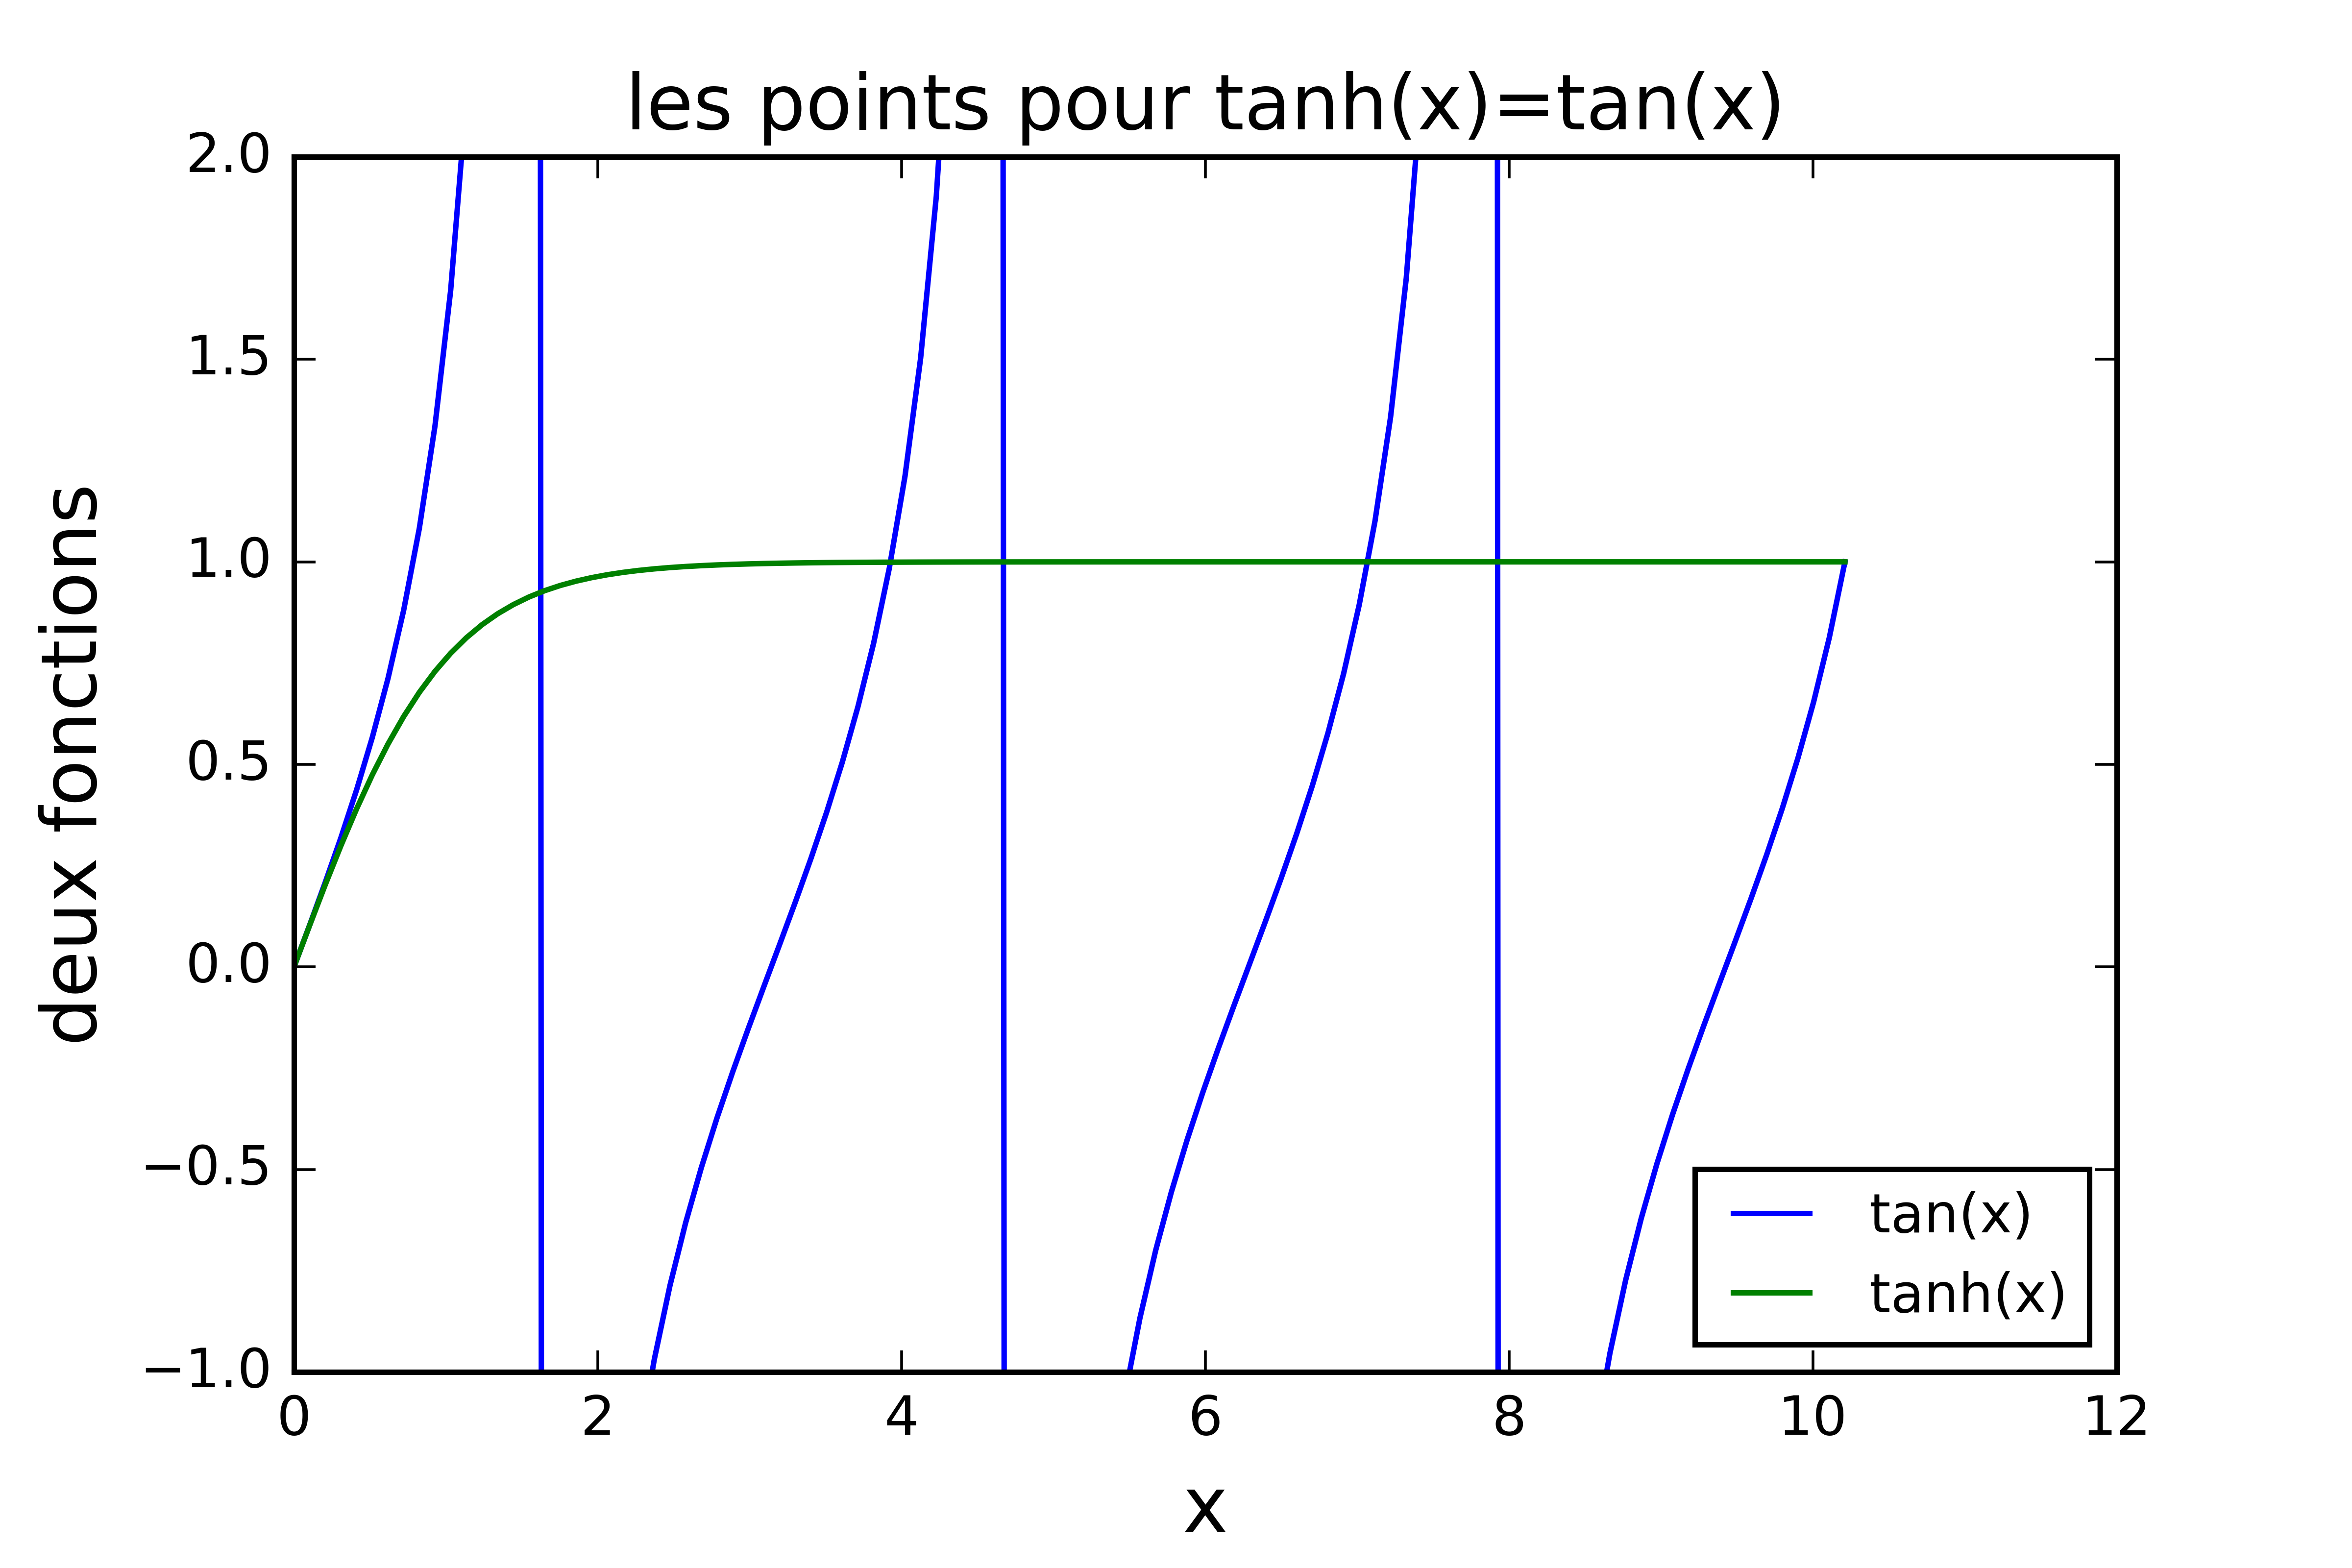
\includegraphics[width=1.0\textwidth]{figuretanh}
\caption{infinité points}
\label{figure1}
\end{figure}

On constate qu'il esixste une infinité de solution , voisines de $\frac{9\pi}{4},\frac{13\pi}{4},\frac{5\pi}{4}$ , etc.

Les valeurs précises peuvent être recherchées numériquement au voisinage de ces valeurs , au moyen d'un programme Matlab très bref :

\begin{center}
for $\gamma$=1:4,
   fzero(@(gamma) tan(gamma)-tanh(gamma) , (4*r*pi-1)/5
\end{center}

On obtient:
\begin{align}
    \gamma_1=3.927\\
    \gamma_2=7.069\\
    \gamma_3=10.210\\
    \gamma_4=13.351\\
    \gamma_5=16.493\\
    \gamma_6= 19.634\\
    \gamma_7=22.776\\
    \gamma_8=25.918\\
    \gamma_9=29.059\\
    \gamma_{10}=32.201\\
    ......\\
    \gamma_r=(4*n*pi-1)/5
\end{align}

A chaque solution $\gamma_r$ corespond une valeur $\omega_r$ de la pulsation:

\begin{equation}
    \omega_r=\frac{\gamma_r^2}{L^2}\sqrt{\frac{EI}{\rho S}}
\end{equation}

\section{Solution générale}
Finalement , la solution générale est :
\begin{equation}
    v(x,t)=\sum\limits_{r=1}^{\infty}\phi_r(x)(E_r\sin{\omega t}+F_r\cos{\omega t)}
\end{equation}

avec:

\begin{equation}
    \left\{
    \begin{array}{r c l}
    \phi_r(x)&=&A\Big(\sinh{(\gamma_r\frac{x}{L})}-\tanh{\gamma_r}\cosh{(\gamma_r\frac{x}{L})}-\sin{(\gamma_r\frac{x}{L})}+\tanh{\gamma_r}\cos{(\gamma_r\frac{x}{L})}\Big)\\
    \omega_r&=&\frac{\gamma_r^2}{L^2}\sqrt{\frac{EI}{\rho S}}\\
    \tanh{\gamma_r}&=&\tan{\gamma_r}\\
    r&=&1,2,3,4......
    \end{array}
    \right.
\end{equation}

%%%%%%%%%%%%%%%%%%%%%%%%%%%%%%%%%%%%%%%%%%%%%%%%%%%%%
\chapter{Analyse et Résultat}

Dans ce chapitre on étude la solution complète avec les conditions initiales .

\section{Premier condition}
condition initiale $v(x,0)=v_0$ 
\subsection{serie de $F_r$}
\begin{align}
    v(x,t)&=\sum\limits_{r=1}^{\infty}\phi_r(x)(E_r\sin{\omega t}+F_r\cos{\omega t)}\\
    v(x,0)&=AF_r\Big(\sinh{(\gamma_r\frac{x}{L})}-\tanh{\gamma_r}\cosh{(\gamma_r\frac{x}{L})}-\sin{(\gamma_r\frac{x}{L})}+\tanh{\gamma_r}\cos{(\gamma_r\frac{x}{L})}\Big)\\
    v(x,0)&=v_0
\end{align}

il reste donc on cherche la serie de $F_r$ dans la équation sommation suivante :

\begin{equation}
    \sum\limits_{r=1}^{\infty}AF_r\Big(\sinh{(\gamma_r\frac{x}{L})}-\tanh{\gamma_r}\cosh{(\gamma_r\frac{x}{L})}-\sin{(\gamma_r\frac{x}{L})}+\tanh{\gamma_r}\cos{(\gamma_r\frac{x}{L})}\Big)=v_0
\end{equation}

\subsection{Transformé de Fourier}

On fait évolution de la fonction au-dessus , à gauche et à droite , on fait intergarale suivante en même temps : 

\begin{equation}
    \int_0^L \Big(\sinh{(\gamma_k\frac{x}{L})}-\tanh{\gamma_k}\cosh{(\gamma_k\frac{x}{L})}-\sin{(\gamma_k\frac{x}{L})}+\tanh{\gamma_k}\cos{(\gamma_k\frac{x}{L})}\Big)\, \mathrm dx\,
\end{equation}
$k$ est une constante.


et on obtient : 

\begin{align}
    &\sum\limits_{r=1}^{\infty}\int_0^L AF_r\Big(\sinh{(\gamma_k\frac{x}{L})}-\tanh{\gamma_k}\cosh{(\gamma_k\frac{x}{L})}-\sin{(\gamma_k\frac{x}{L})}+\tanh{\gamma_k}\cos{(\gamma_k\frac{x}{L})}\Big)\\
    &\,\Big(\sinh{(\gamma_r\frac{x}{L})}-\tanh{\gamma_r}\cosh{(\gamma_r\frac{x}{L})}-\sin{(\gamma_r\frac{x}{L})}+\tanh{\gamma_r}\cos{(\gamma_r\frac{x}{L})}\Big)\mathrm dx\\
    &=\int_0^L v_0\Big(\sinh{(\gamma_k\frac{x}{L})}-\tanh{\gamma_k}\cosh{(\gamma_k\frac{x}{L})}-\sin{(\gamma_k\frac{x}{L})}+\tanh{\gamma_k}\cos{(\gamma_k\frac{x}{L})}\Big)\,\mathrm dx
\end{align}
 
On étude le fonction au dessus , on trouve si $r$ est différent que $k$:
\begin{align}
    \int_0^L \Big(\sinh{(\gamma_k\frac{x}{L})}-\tanh{\gamma_k}\cosh{(\gamma_k\frac{x}{L})}-\sin{(\gamma_k\frac{x}{L})}+\tanh{\gamma_k}\cos{(\gamma_k\frac{x}{L})}\Big)\\
    \Big(\sinh{(\gamma_r\frac{x}{L})}-\tanh{\gamma_r}\cosh{(\gamma_r\frac{x}{L})}-\sin{(\gamma_r\frac{x}{L})}+\tanh{\gamma_r}\cos{(\gamma_r\frac{x}{L})}\Big)\mathrm dx=0
\end{align}

si $r=k$:
\begin{align}
    \int_0^L \Big(\sinh{(\gamma_k\frac{x}{L})}-\tanh{\gamma_k}\cosh{(\gamma_k\frac{x}{L})}-\sin{(\gamma_k\frac{x}{L})}+\tanh{\gamma_k}\cos{(\gamma_k\frac{x}{L})}\Big)\\
    \Big(\sinh{(\gamma_r\frac{x}{L})}-\tanh{\gamma_r}\cosh{(\gamma_r\frac{x}{L})}-\sin{(\gamma_r\frac{x}{L})}+\tanh{\gamma_r}\cos{(\gamma_r\frac{x}{L})}\Big)\mathrm dx=L
\end{align}

donc à gauche de signe égale , on a : $ALF_k$


et a droite de signe égale , on a :


\begin{align}
    \int_0^L v_0\Big(\sinh{(\gamma_k\frac{x}{L})}-\tanh{\gamma_k}\cosh{(\gamma_k\frac{x}{L})}-\sin{(\gamma_k\frac{x}{L})}+\tanh{\gamma_k}\cos{(\gamma_k\frac{x}{L})}\Big)\mathrm dx\\
    =\frac{L v_0\,\Big(\cos(\gamma_k)+\cosh(\gamma_k)+\tanh(\gamma_k)(\sin(\gamma_k)-\sinh(\gamma_k))-2\Big)}{\gamma_k}
\end{align}


et finalement on trouve $F_k$:

\begin{equation}
    F_k=\frac{v_0}{A\,\gamma_k}\,\Big(\cos(\gamma_k)+\cosh(\gamma_k)+\tanh(\gamma_k)(\sin(\gamma_k)-\sinh(\gamma_k))-2\Big)
\end{equation}

k et r sont constantes 1,2 ,3......

\begin{equation}
    F_r=\frac{v_0}{A\,\gamma_r}\,\Big(\cos(\gamma_r)+\cosh(\gamma_r)+\tanh(\gamma_r)(\sin(\gamma_r)-\sinh(\gamma_r))-2\Big)
\end{equation}


\section{Deuxième condition}

dans le deuxième condition on a $\frac{\partial v(x,0)}{\partial t}=0$

\subsection{Derivée partiel d'équation}

On fait la dérivée partielle de $v(x,t)$ sur $t$

\begin{align}
    \frac{\partial v(x,t)}{\partial t}=\  &AEw\cos{(\omega t)}\Big(\sinh{(\gamma\frac{x}{L})}-\tanh{\gamma}\cosh{(\gamma\frac{x}{L})}-\sin{(\gamma\frac{x}{L})}+\tanh{\gamma}\cos{(\gamma\frac{x}{L})}\Big)\\&-AFw\sin{(\omega t)}\Big(\sinh{(\gamma\frac{x}{L})}-\tanh{\gamma}\cosh{(\gamma\frac{x}{L})}-\sin{(\gamma\frac{x}{L})}+\tanh{\gamma}\cos{(\gamma\frac{x}{L})}\Big)
\end{align}


\subsection{Nulle  de derivation}

On a toujour l'équation suivante :

\begin{equation}
    \frac{\partial v(x,0)}{\partial t}=AE_r\Big(\sinh{(\gamma_r\frac{x}{L})}-\tanh{\gamma_r}\cosh{(\gamma_r\frac{x}{L})}-\sin{(\gamma_r\frac{x}{L})}+\tanh{\gamma_r}\cos{(\gamma_r\frac{x}{L})}\Big)=0
\end{equation}

Donc evidment , $E_r=0$ pour tous les $r$ .


%%%%%%%%%+++++++++++++++++++++++++++++++++++%%%%%%%%%%%%%%%%%%%%ù
\section{Solution complète}

Avec les conditions initiales on arrive :

\begin{equation}
    \left\{
    \begin{array}{r c l}
         v(x,t)&=&\sum\limits_{r=1}^{\infty} AF_r\cos(\omega_r t)\Big(\sinh{(\gamma_r\frac{x}{L})}-\tanh{\gamma_r}\cosh{(\gamma_r\frac{x}{L})}-\sin{(\gamma_r\frac{x}{L})}+\tanh{\gamma_r}\cos{(\gamma_r\frac{x}{L})}\Big)\\
         AF_r&=&\frac{v_0}{\gamma_r}\,\Big(\cos(\gamma_r)+\cosh(\gamma_r)+\tanh(\gamma_r)(\sin(\gamma_r)-\sinh(\gamma_r))-2\Big)\\
         \omega_r&=&\frac{\gamma_r^2}{L^2}\sqrt{\frac{EI}{\rho S}}\\
         E_r&=&0
    \end{array}
    \right.
\end{equation}

%%%%%%%%%%%%%%%%%%%%%%%%%%%%%%%%%%%%%%%%%%%%%%%%%%%%%%%%%%%%
\chapter{ Prénsatations Graphiques}

On untilise Jupyter Nootbook pour prensenter les graphiques : pour toutes les valeurs en bosoin , on note 1 , 
\begin{align}
    E=1\\
    L=1\\
    I=1\\
    rho=1\\
    S=1
\end{align}

\section{Graphiques temps fixé}

\subsection{Mode 1 ($\gamma=\gamma_1$)}

$\gamma_1=3.927$ :

\begin{figure}[H]
\centering
%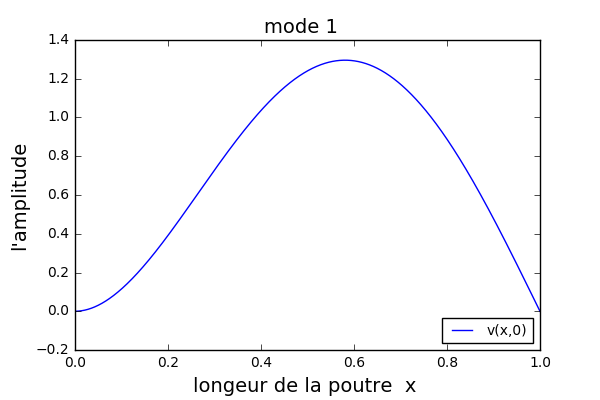
\includegraphics[width=1.0\textwidth]{mode1}
\label{figure2}
\caption{t=0 mode 1}
\end{figure}

\subsection{Mode 2 ($\gamma=\gamma_2$)}

$\gamma_2=7.069$ :

\begin{figure}[H]
\centering
%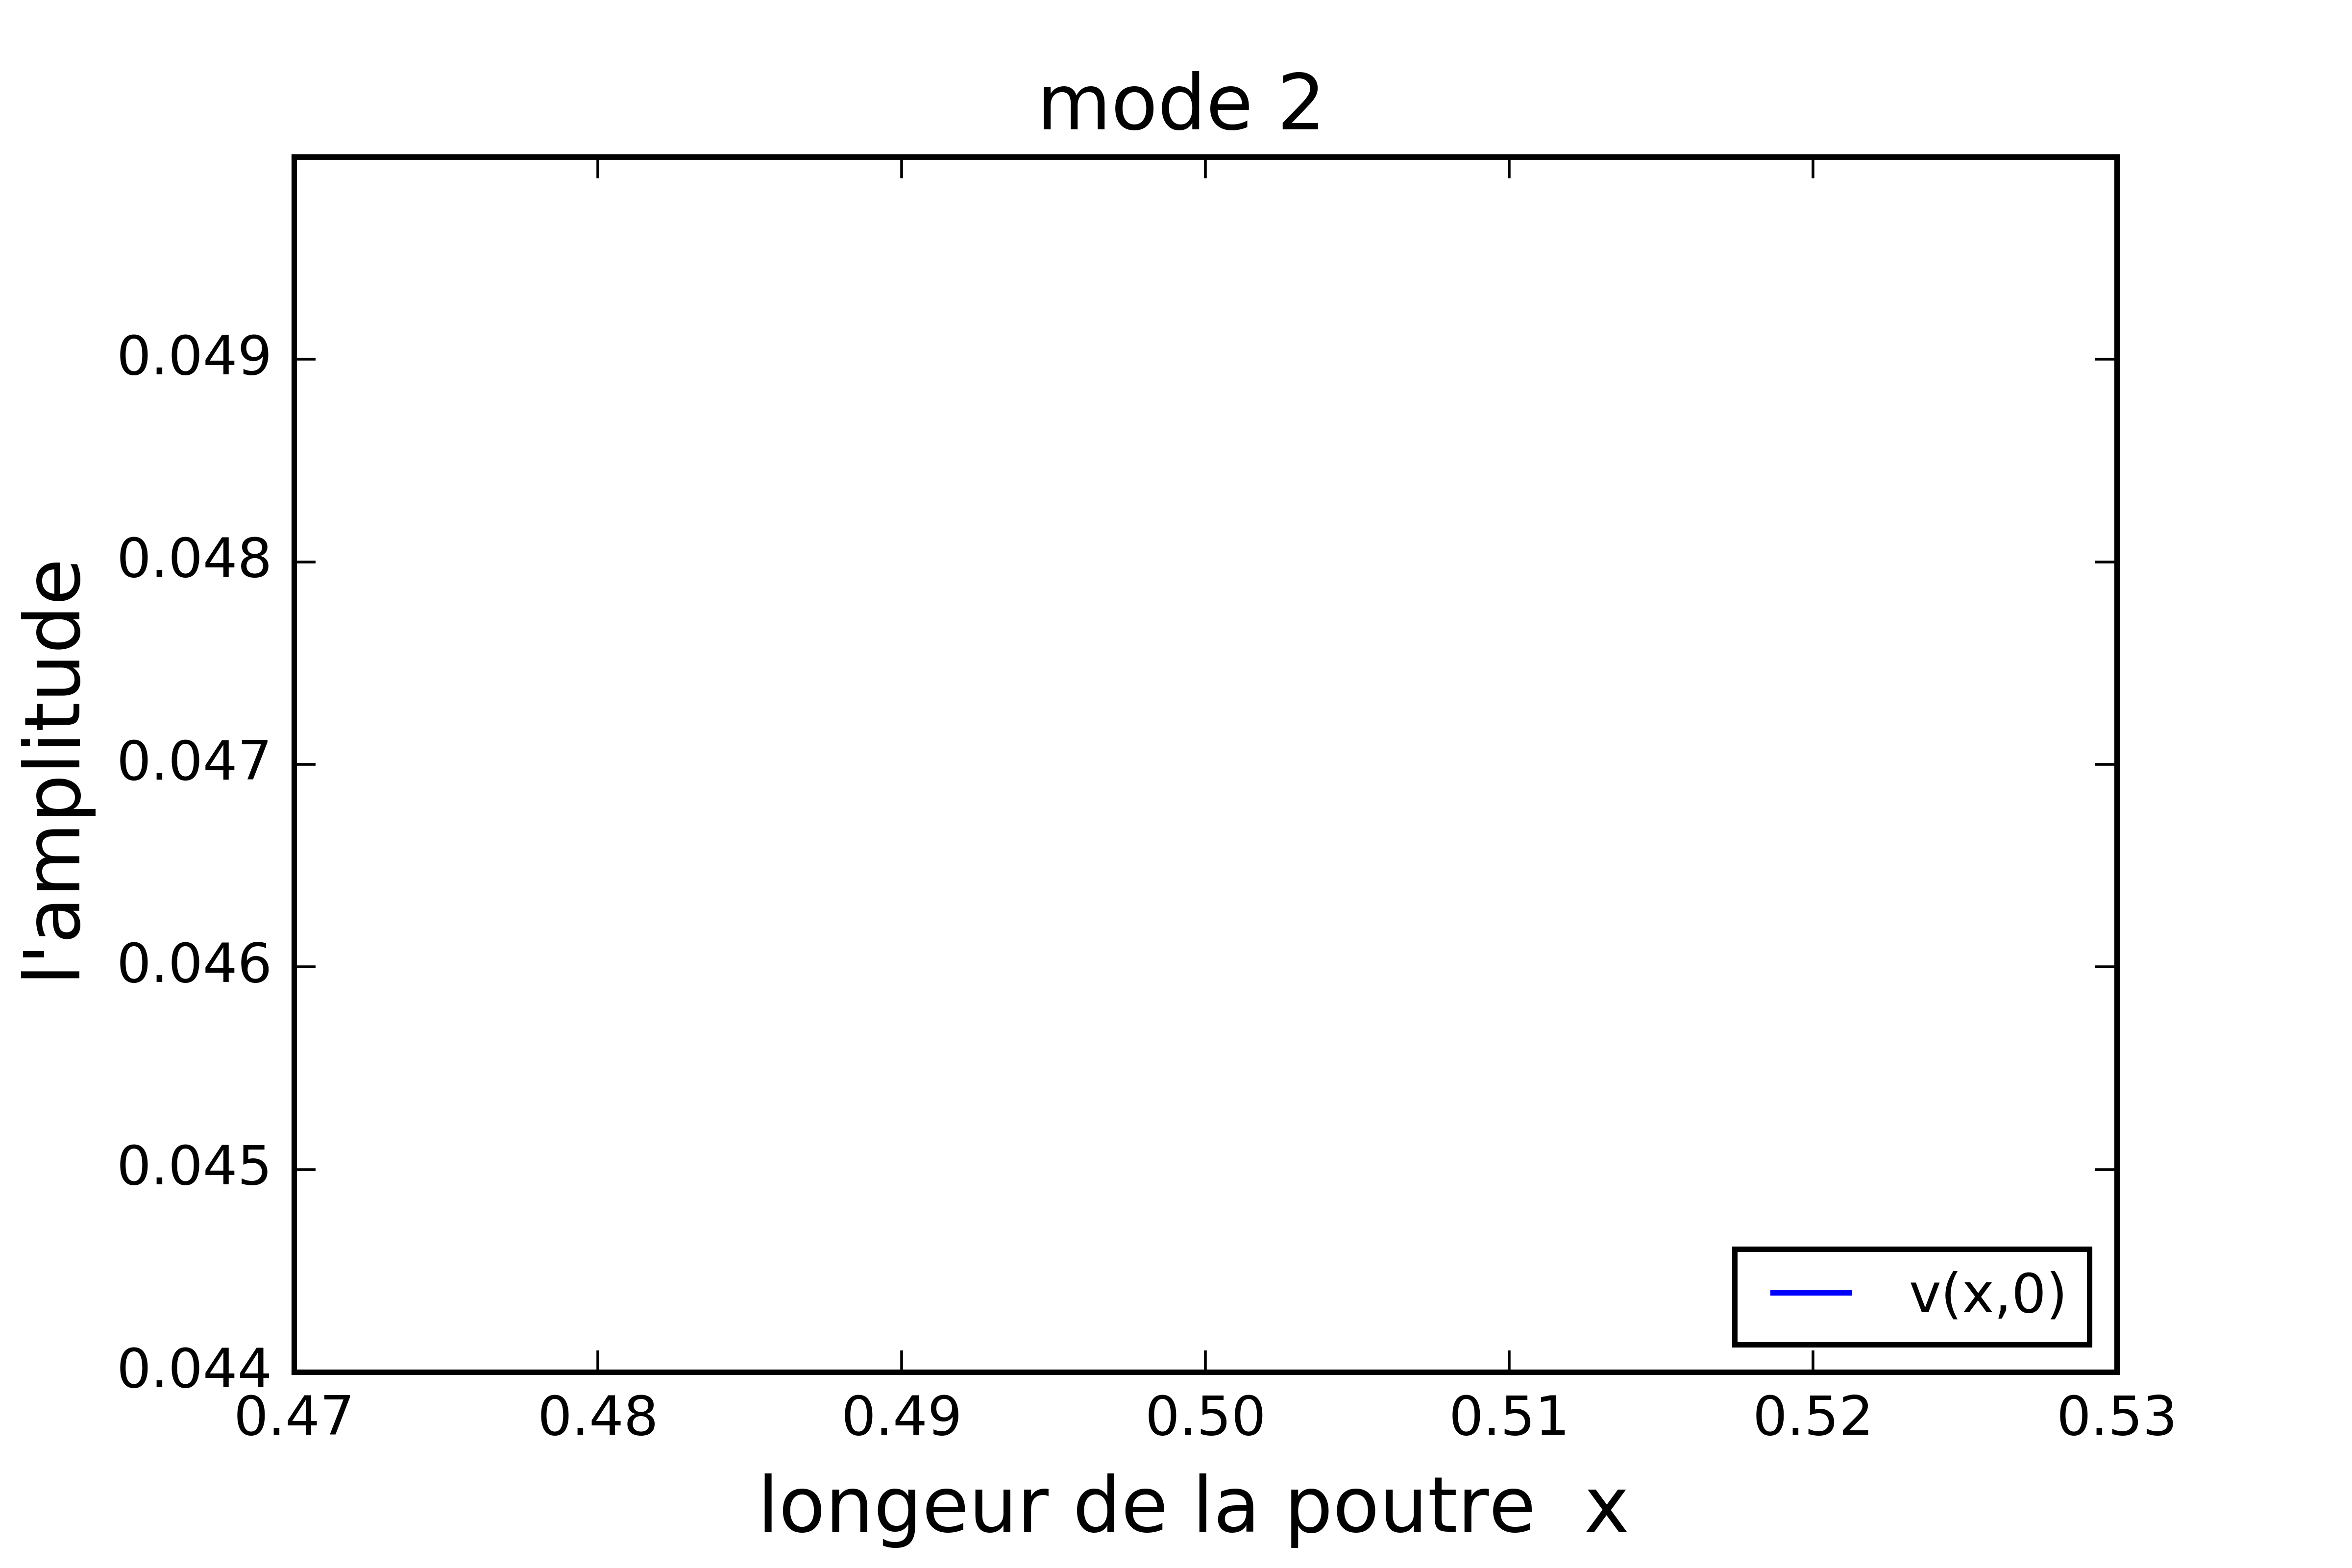
\includegraphics[width=1.0\textwidth]{mode2}
\label{figure3}
\caption{t=0 mode 2}
\end{figure}

\subsection{V(x,0) total pour $\gamma_1$ et $\gamma_2$}

\begin{figure}[H]
\centering
%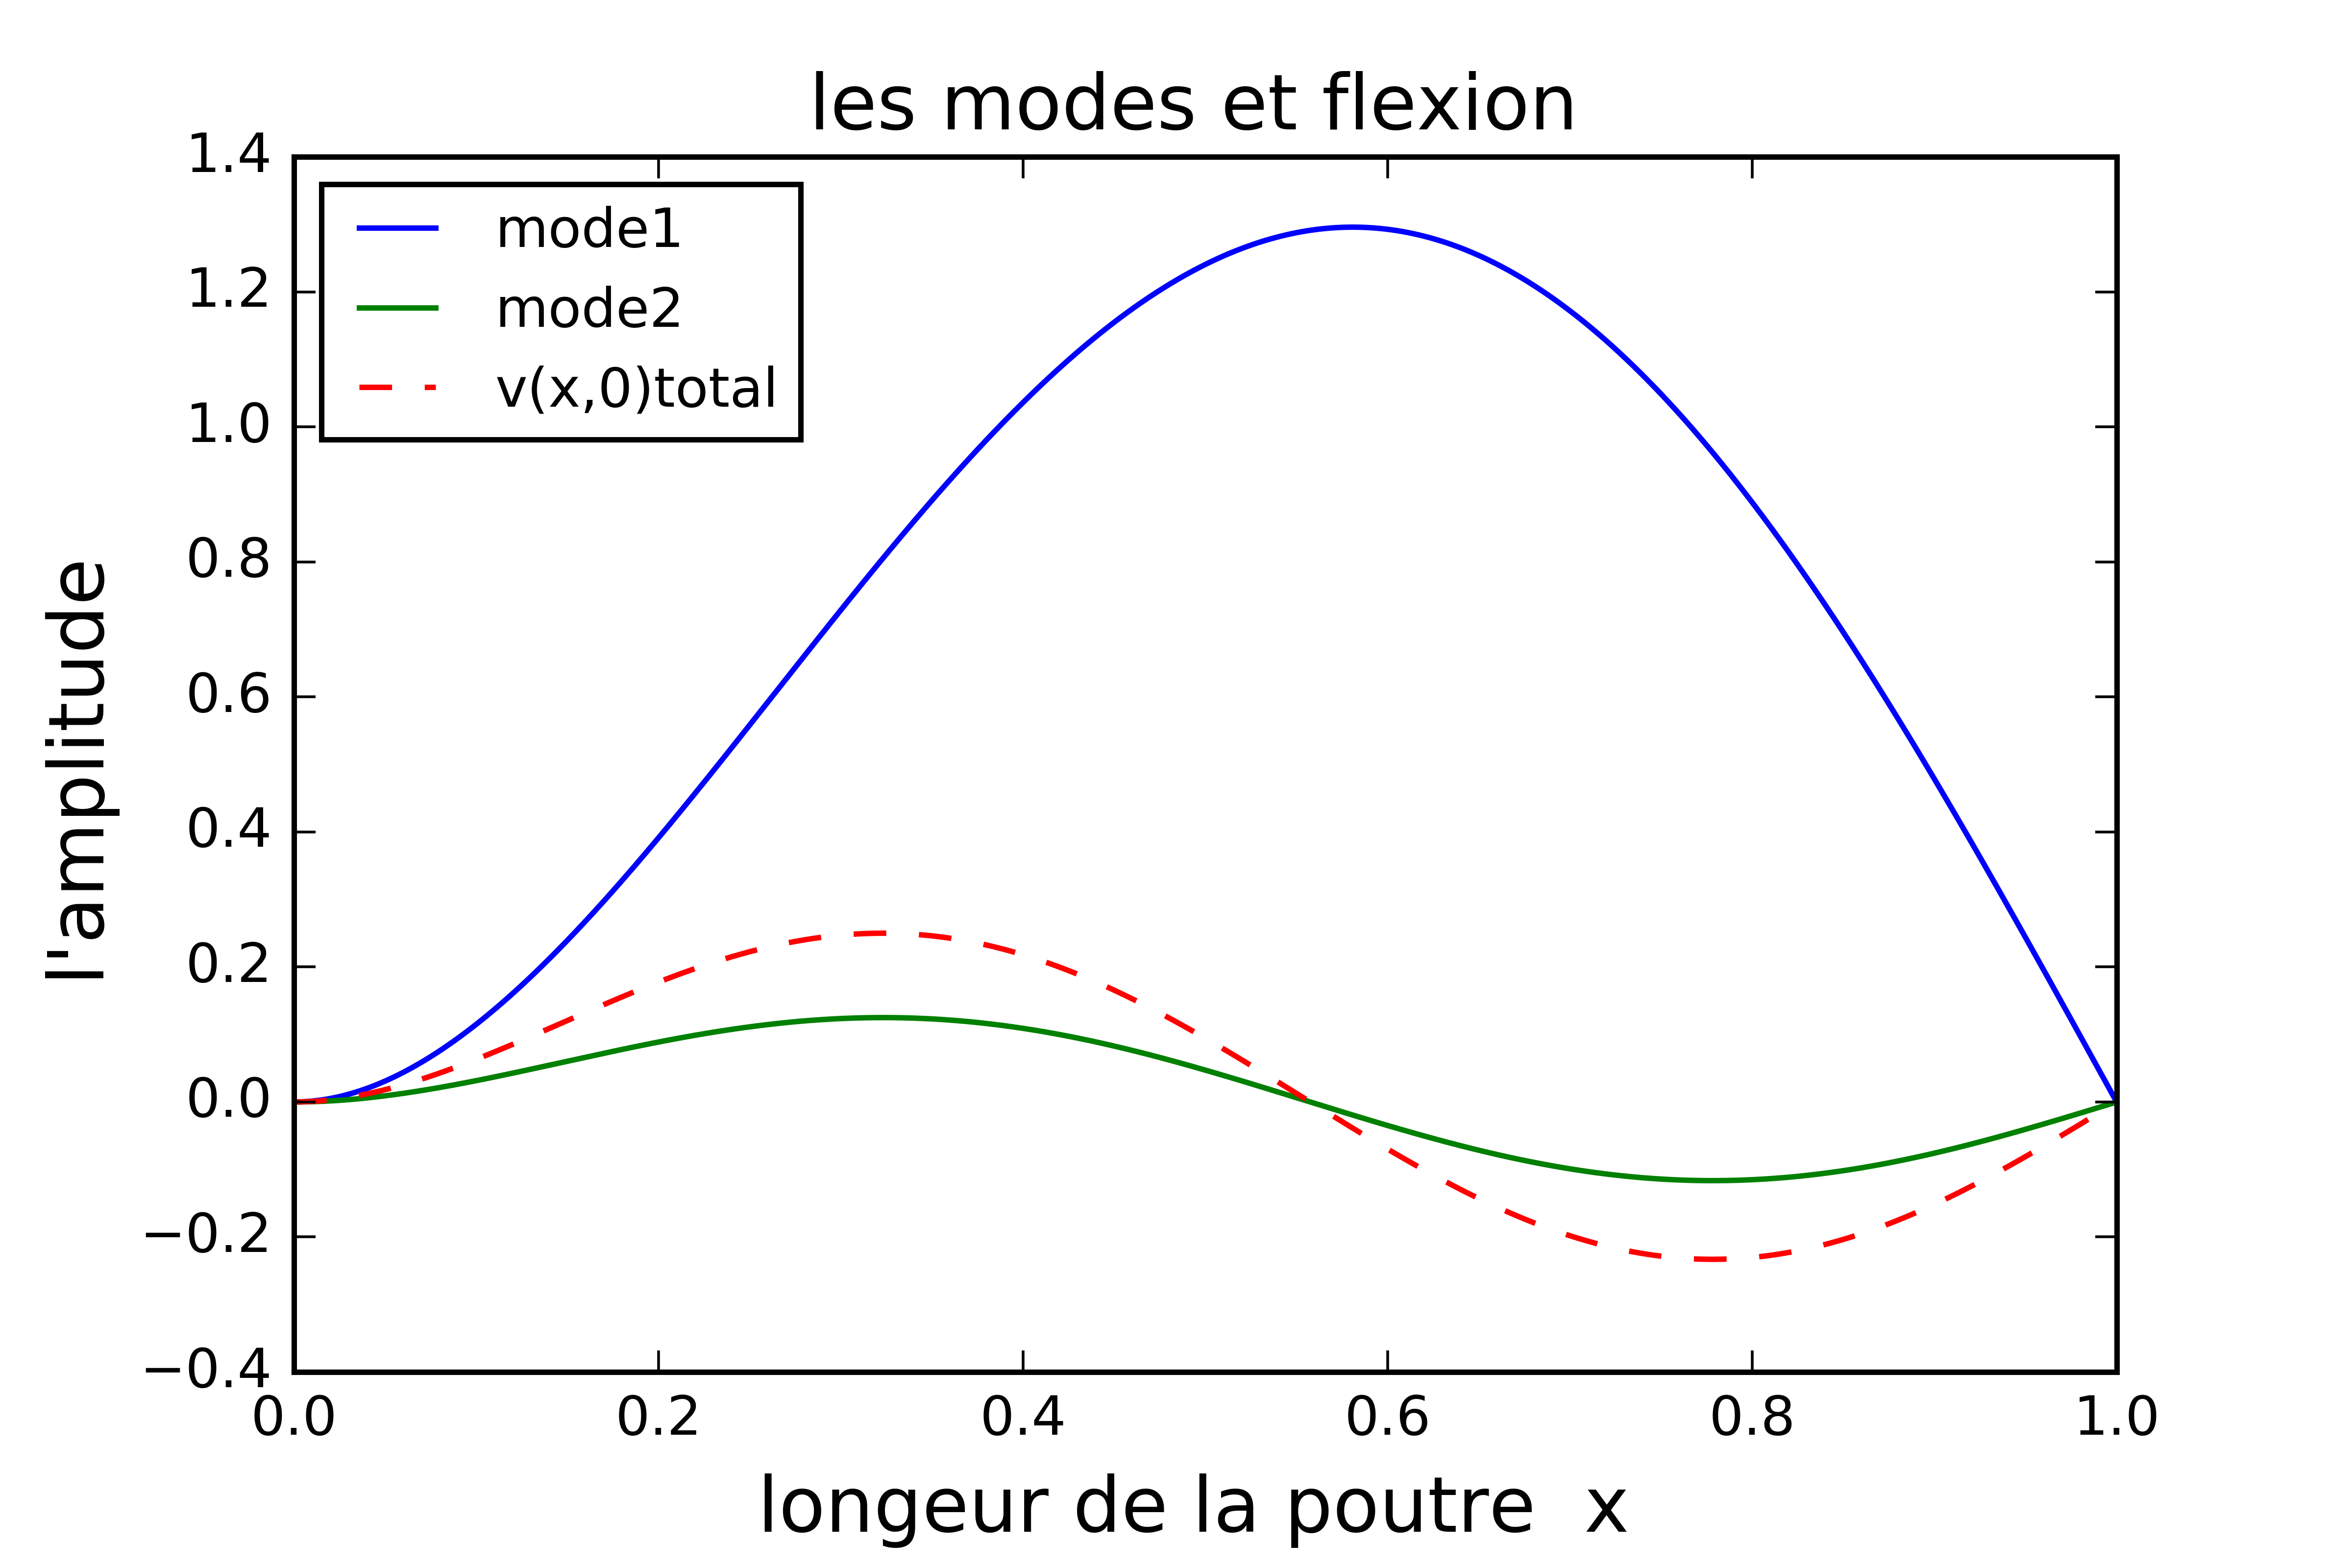
\includegraphics[width=1.0\textwidth]{modee2}
\label{figure4}
\caption{2 modes et vibrations}
\end{figure}

\subsection{Mode 5 ($\gamma=\gamma_5$)}

$\gamma_5=16.493$ :

\begin{figure}[H]
\centering
%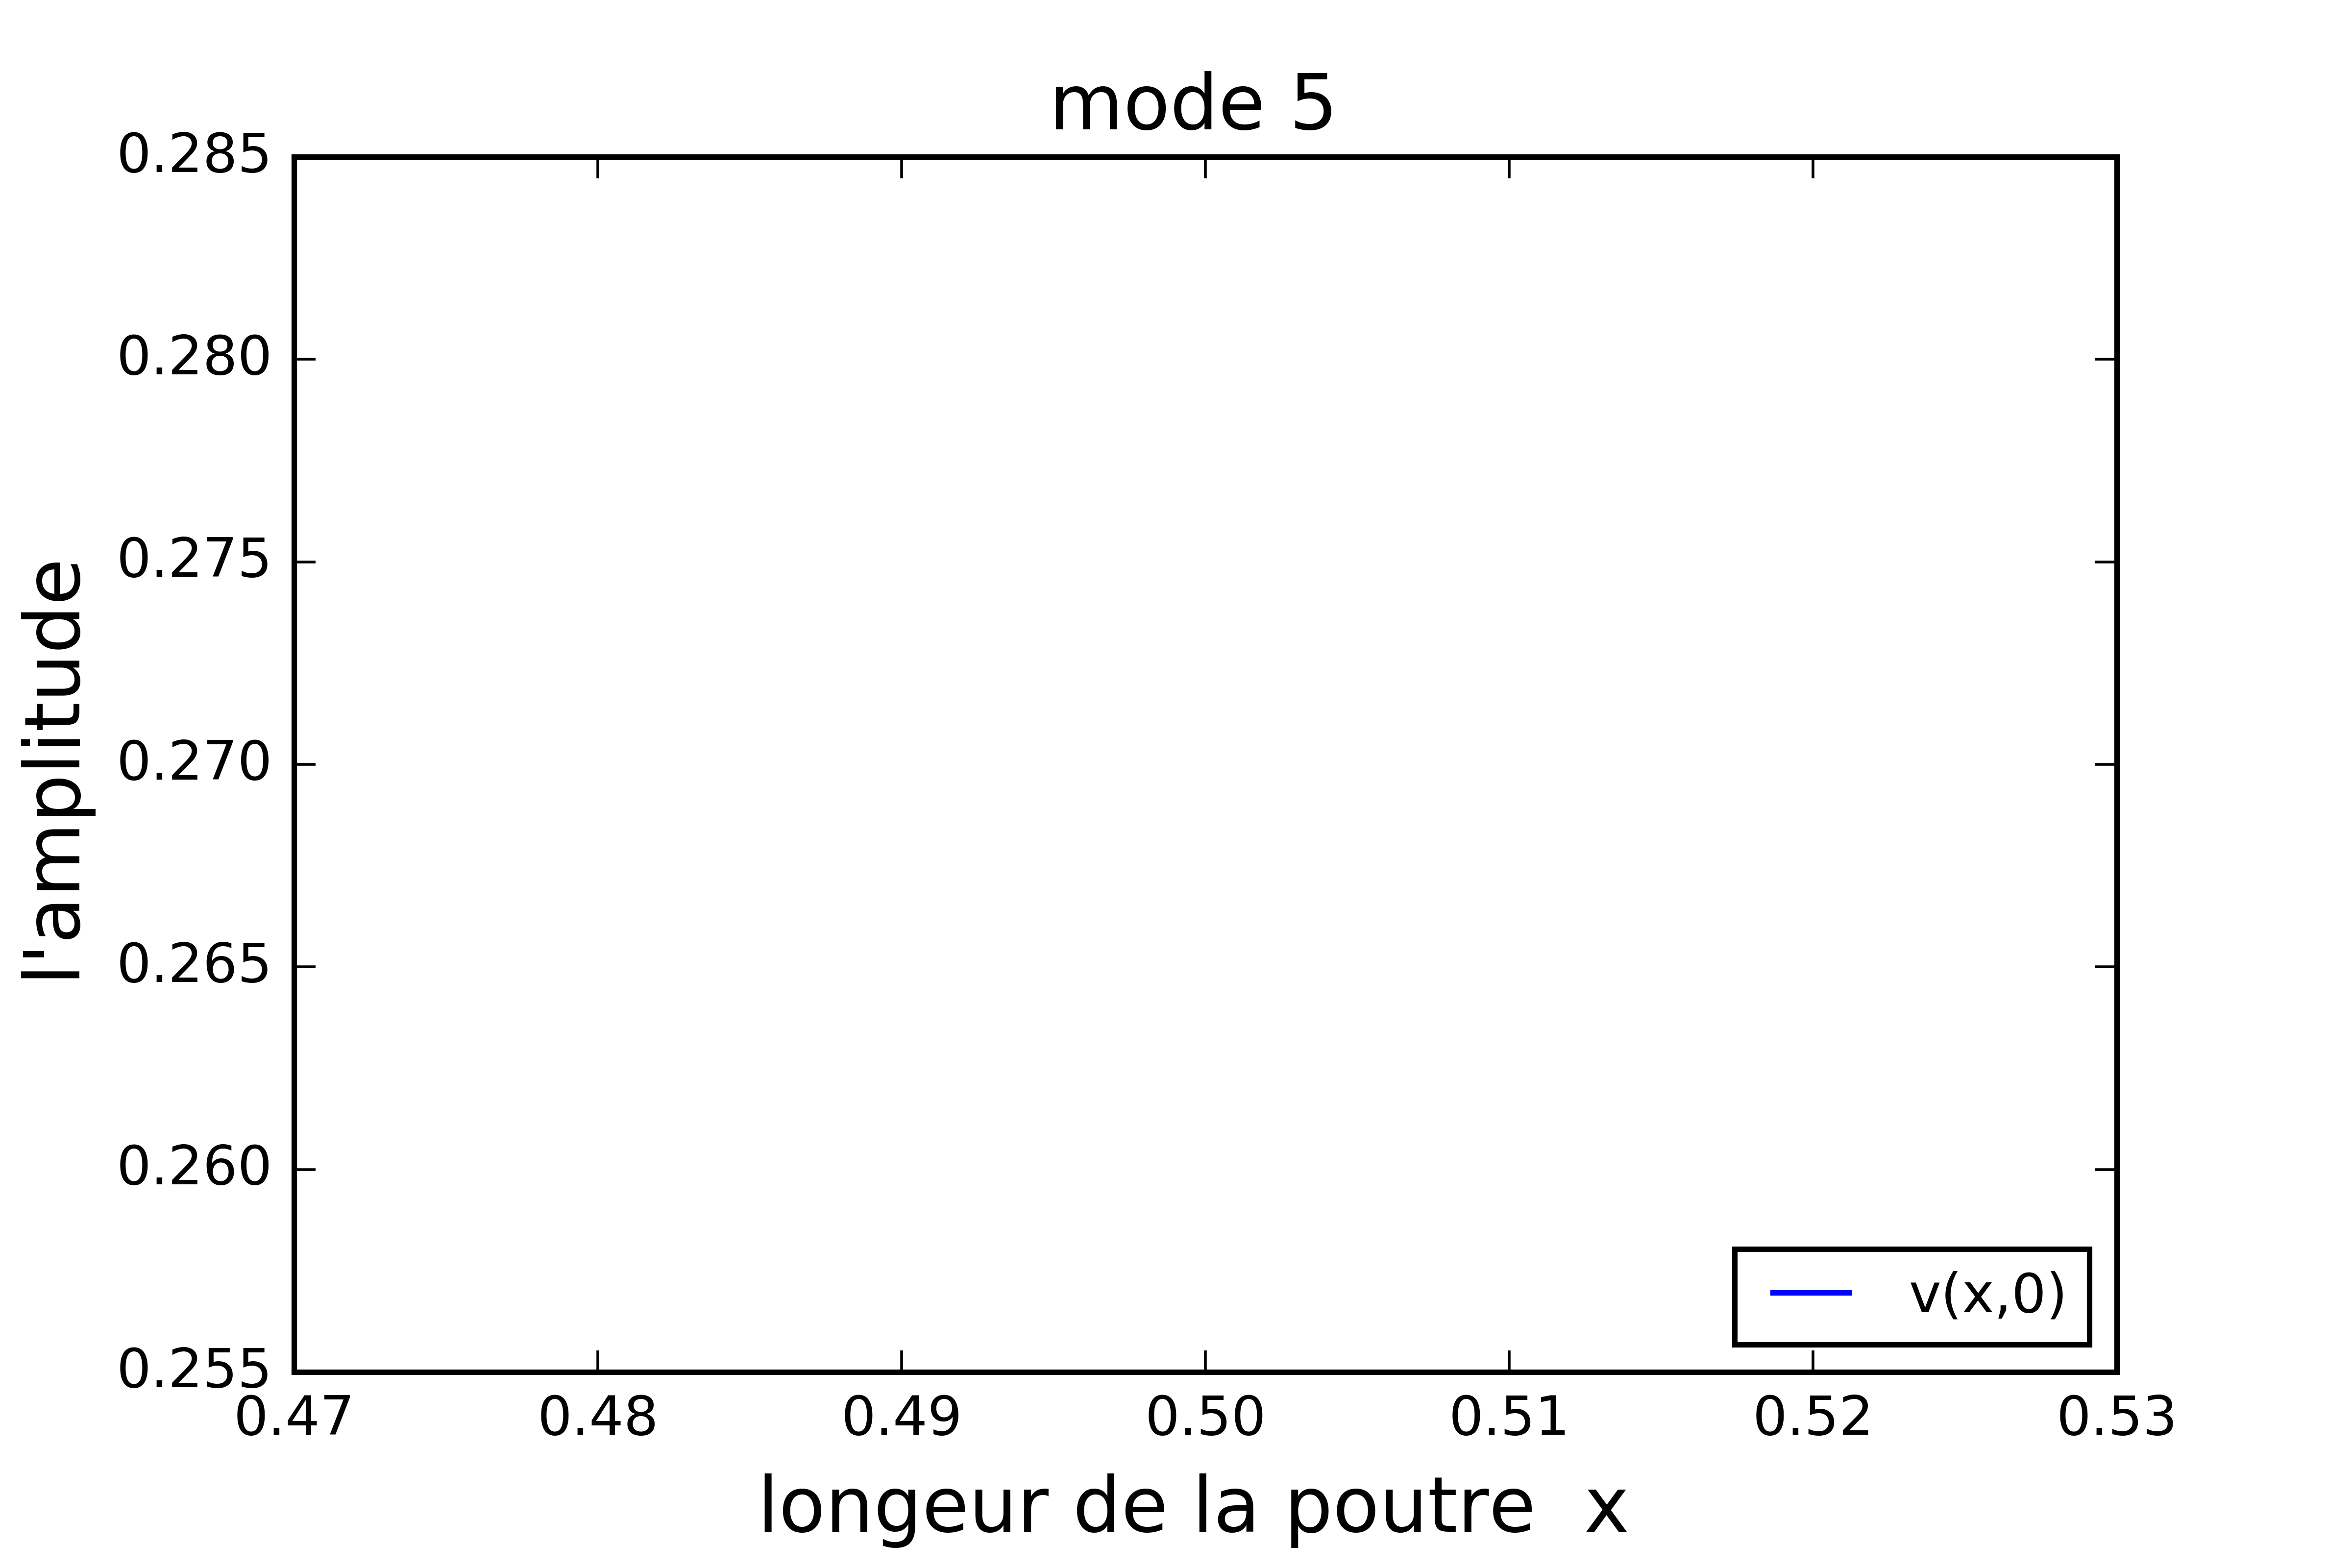
\includegraphics[width=1.0\textwidth]{mode5}
\label{figure5}
\caption{t=0 mode 5}
\end{figure}

\subsection{V(x,0) total pour $\gamma_1$,$\gamma_2$,$\gamma_3$,$\gamma_4$,$\gamma_5$}


\begin{figure}[H]
\centering
%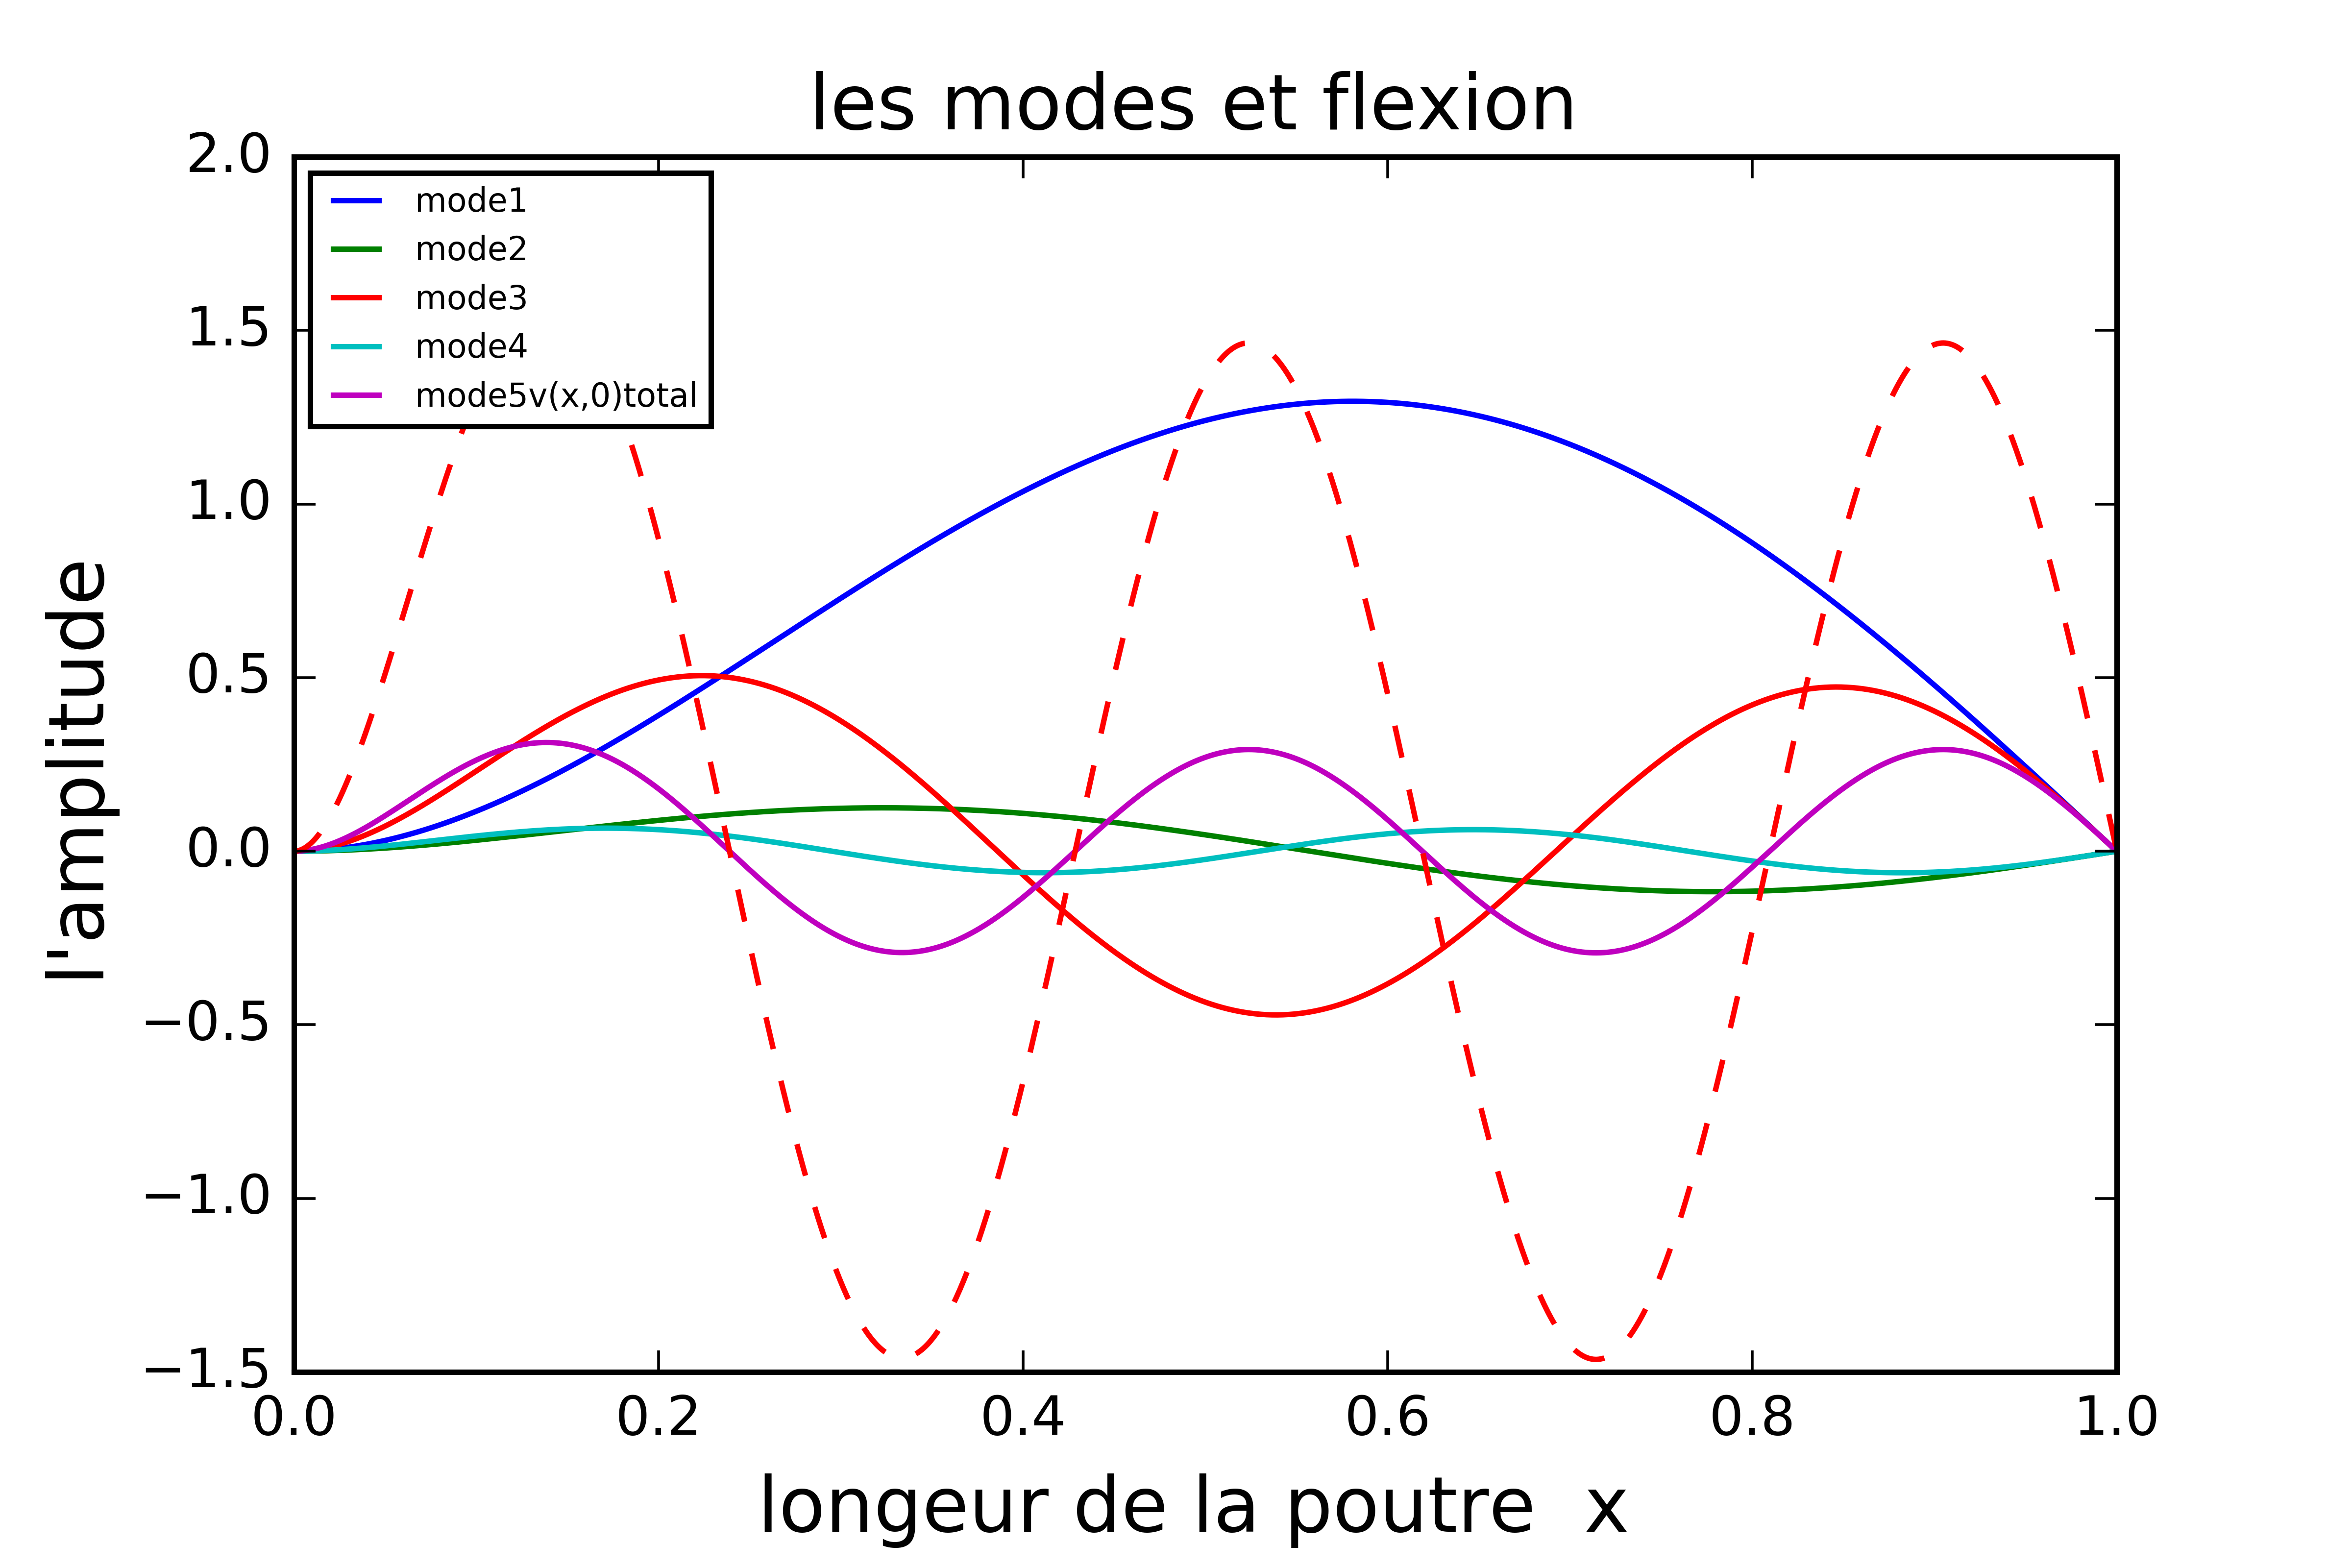
\includegraphics[width=1.0\textwidth]{modee5}
\label{figure6}
\caption{5 modes et vibrations}
\end{figure}


\section{Graphiques position fixé}

On choisi pa position milieu $x=0.5$ pour présenter :


\subsection{Mode1 du temps }

\begin{figure}[H]
\centering
%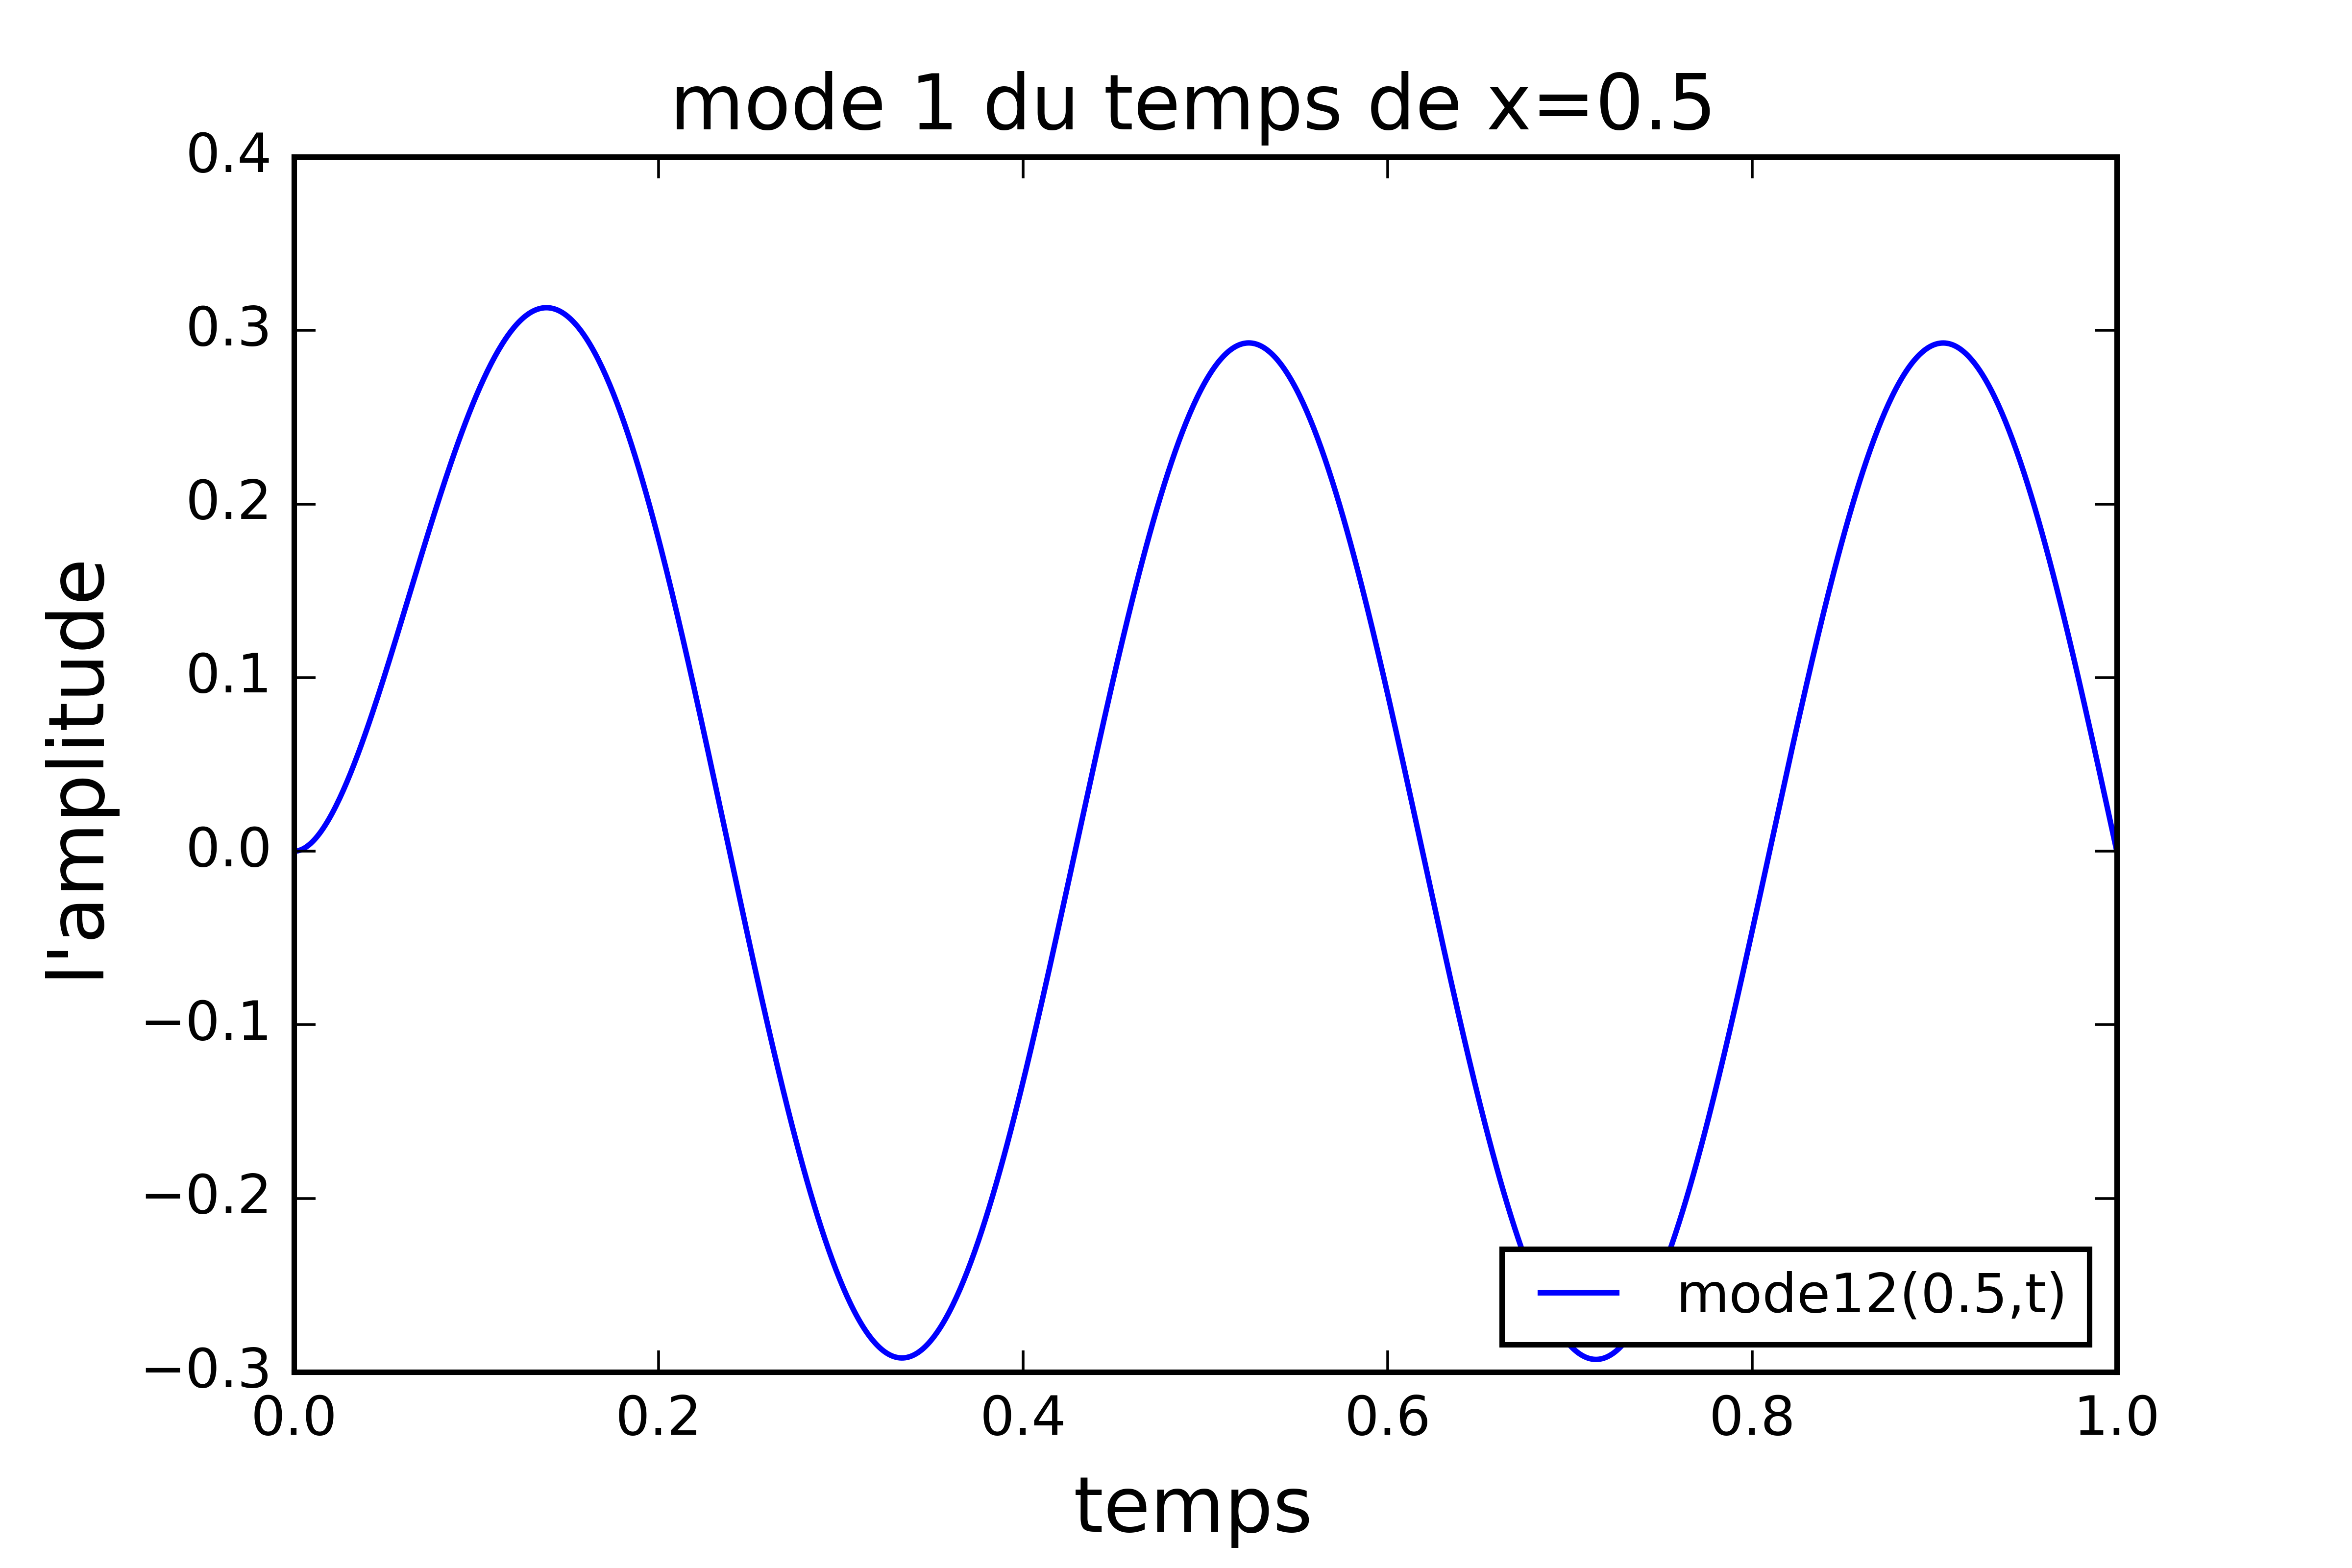
\includegraphics[width=1.0\textwidth]{mode1t}
\label{figure7}
\caption{mode1 du temps}
\end{figure}

\subsection{Mode2 du temps }

\begin{figure}[H]
\centering
%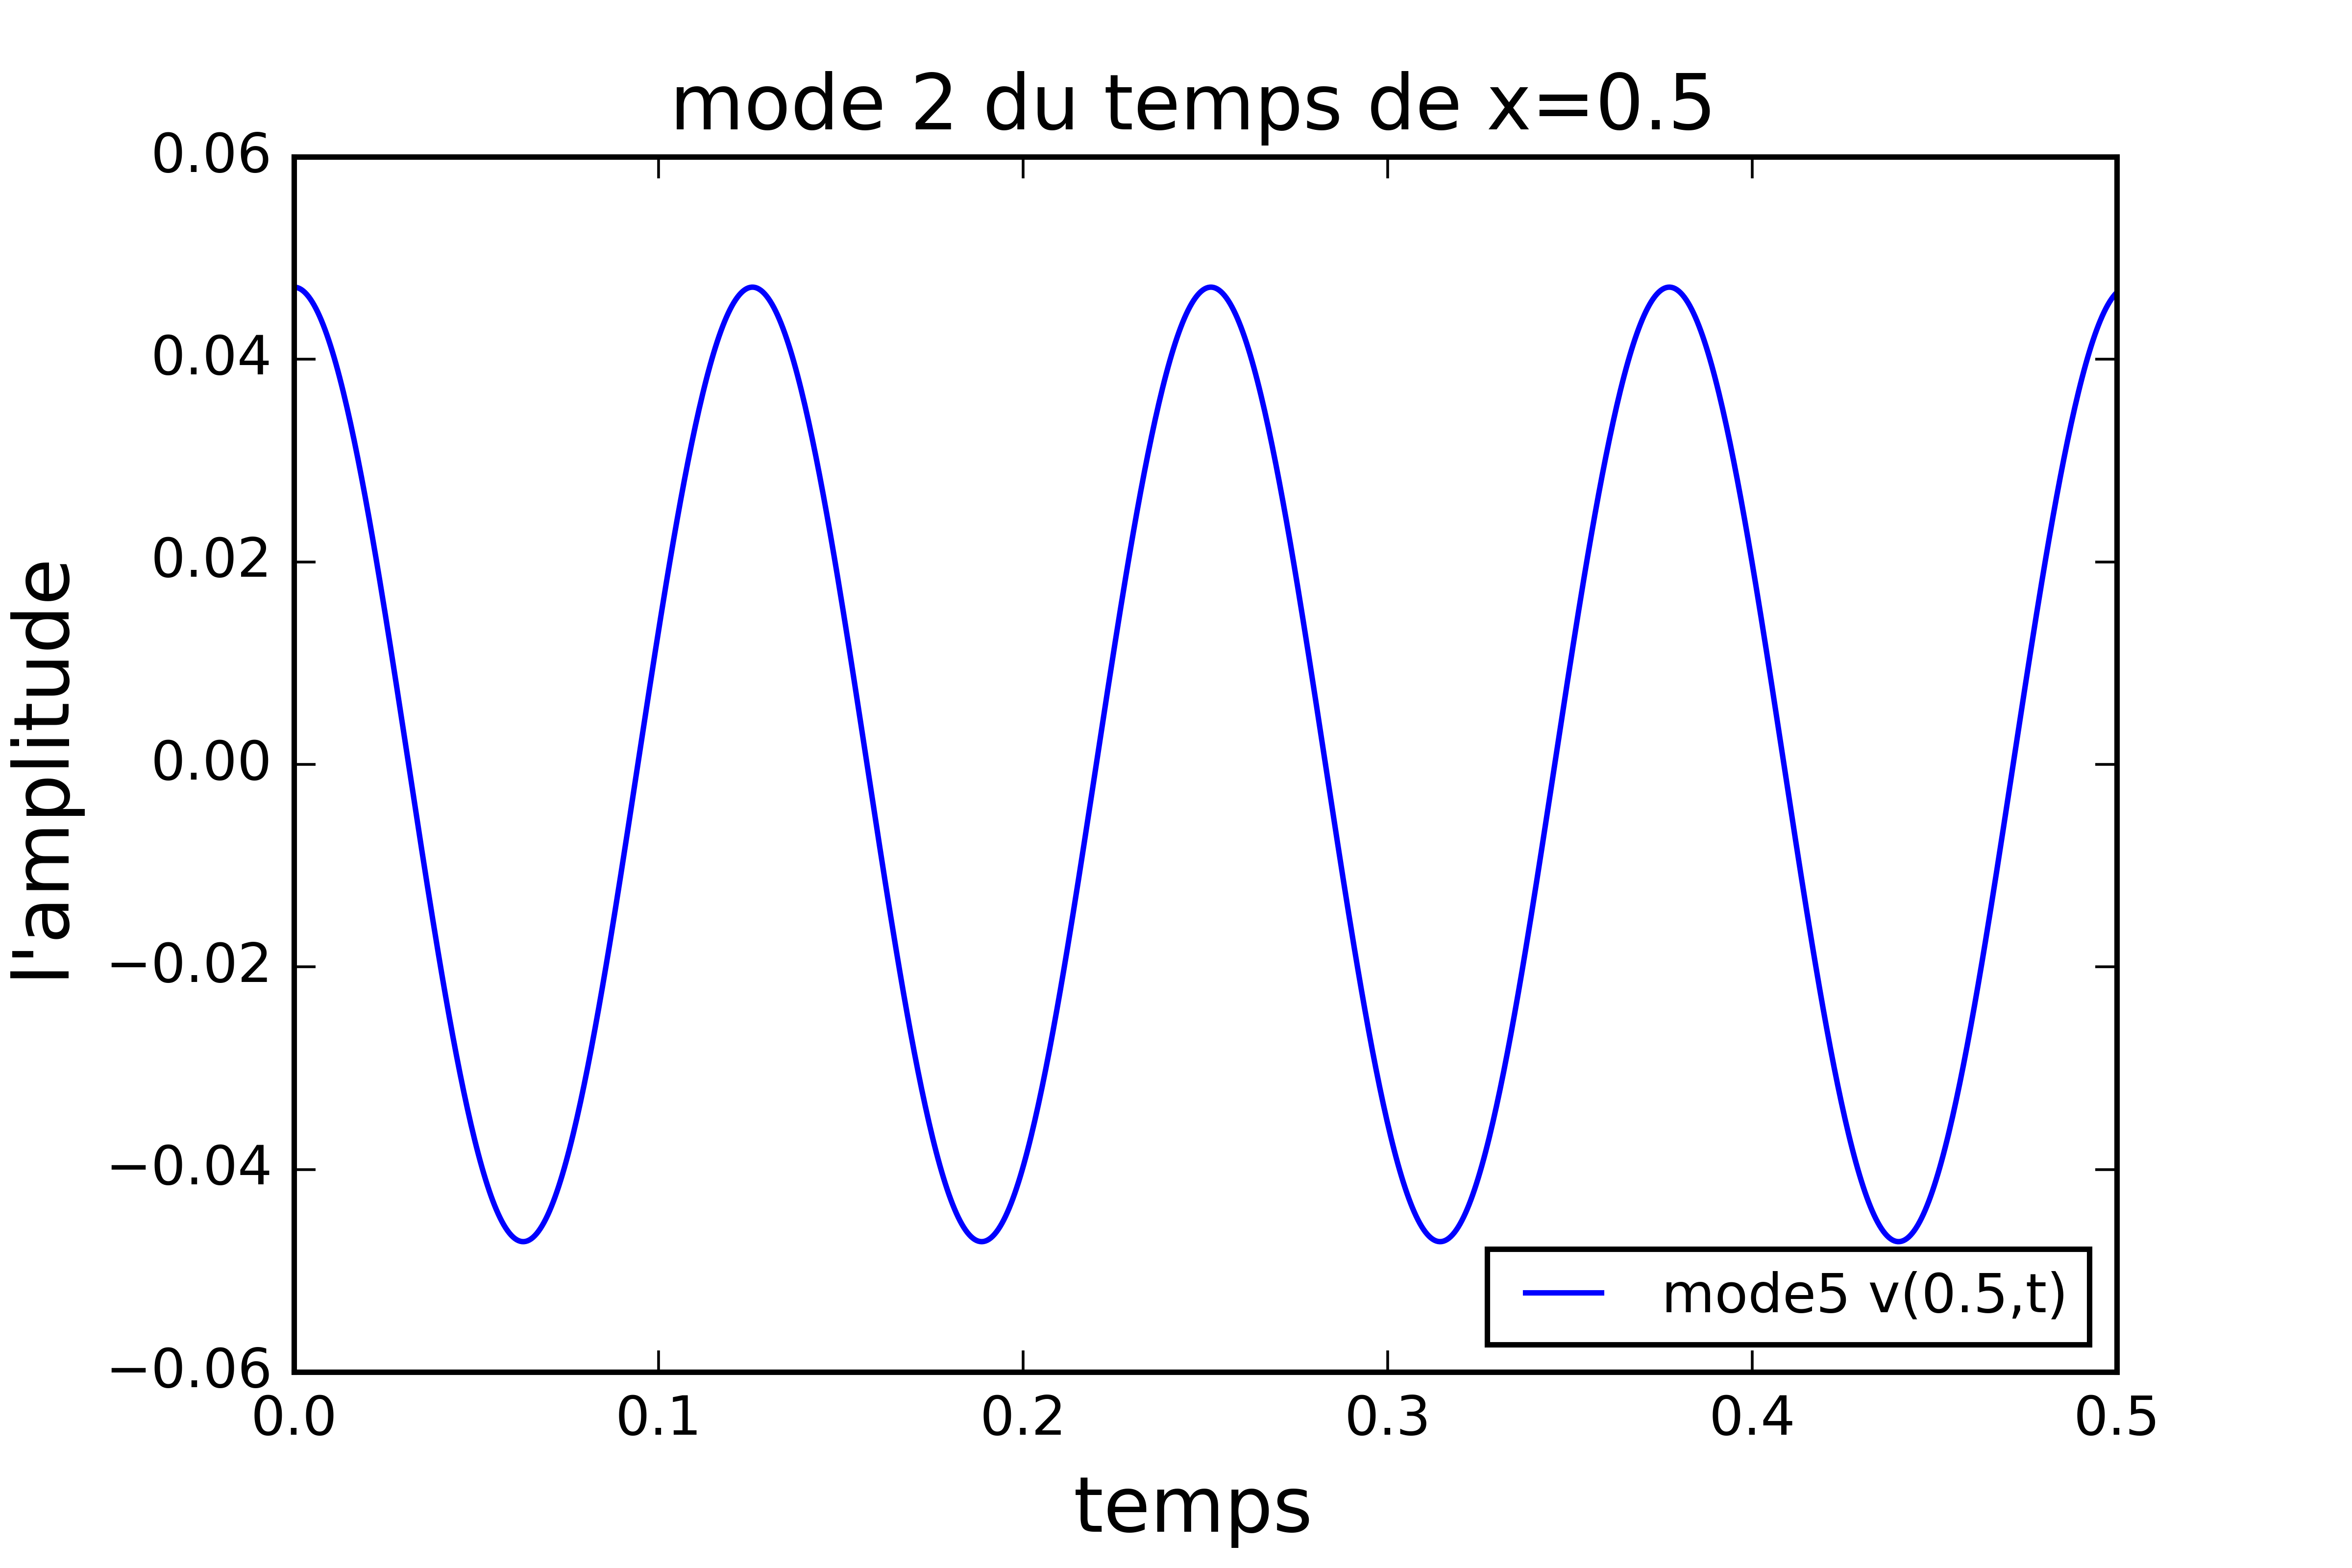
\includegraphics[width=1.0\textwidth]{mode2t}
\label{figure8}
\caption{mode2 du temps}
\end{figure}

\subsection{Viration2 total du temps }

\begin{figure}[H]
\centering
%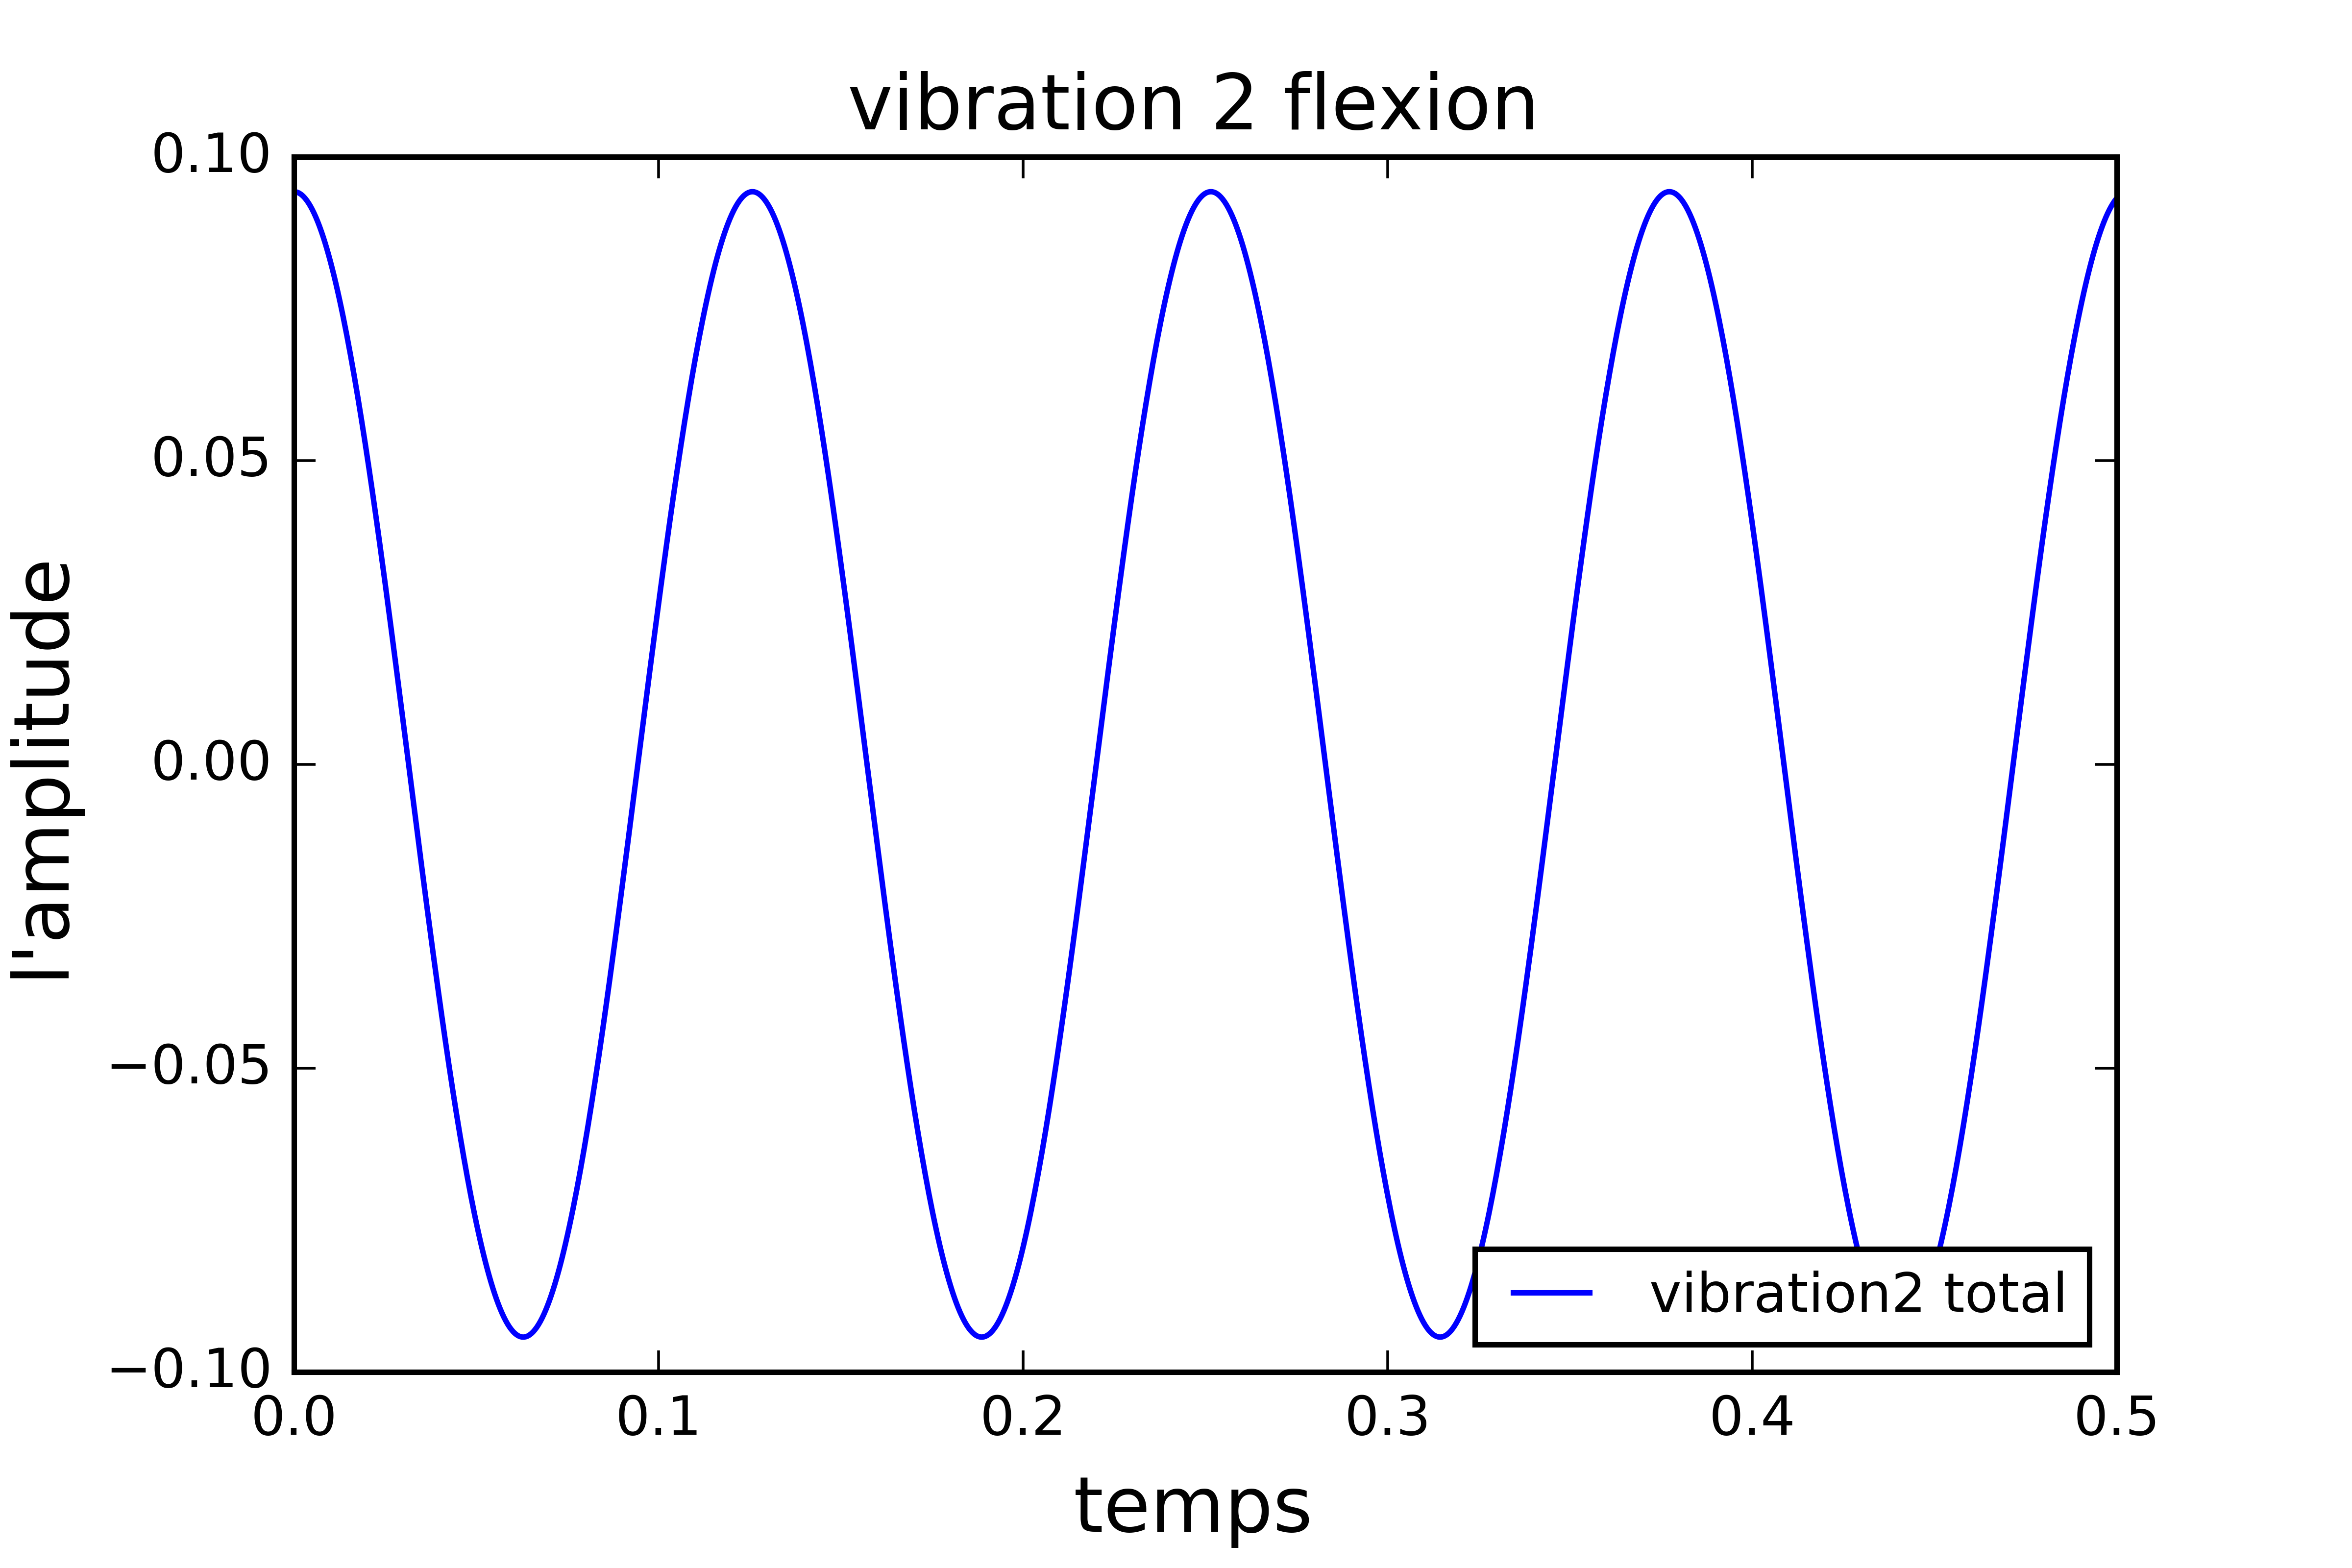
\includegraphics[width=1.0\textwidth]{modee2vt}
\label{figure9}
\caption{vibration2 du temps}
\end{figure}

\subsection{Viration5 total du temps }

\begin{figure}[H]
\centering
%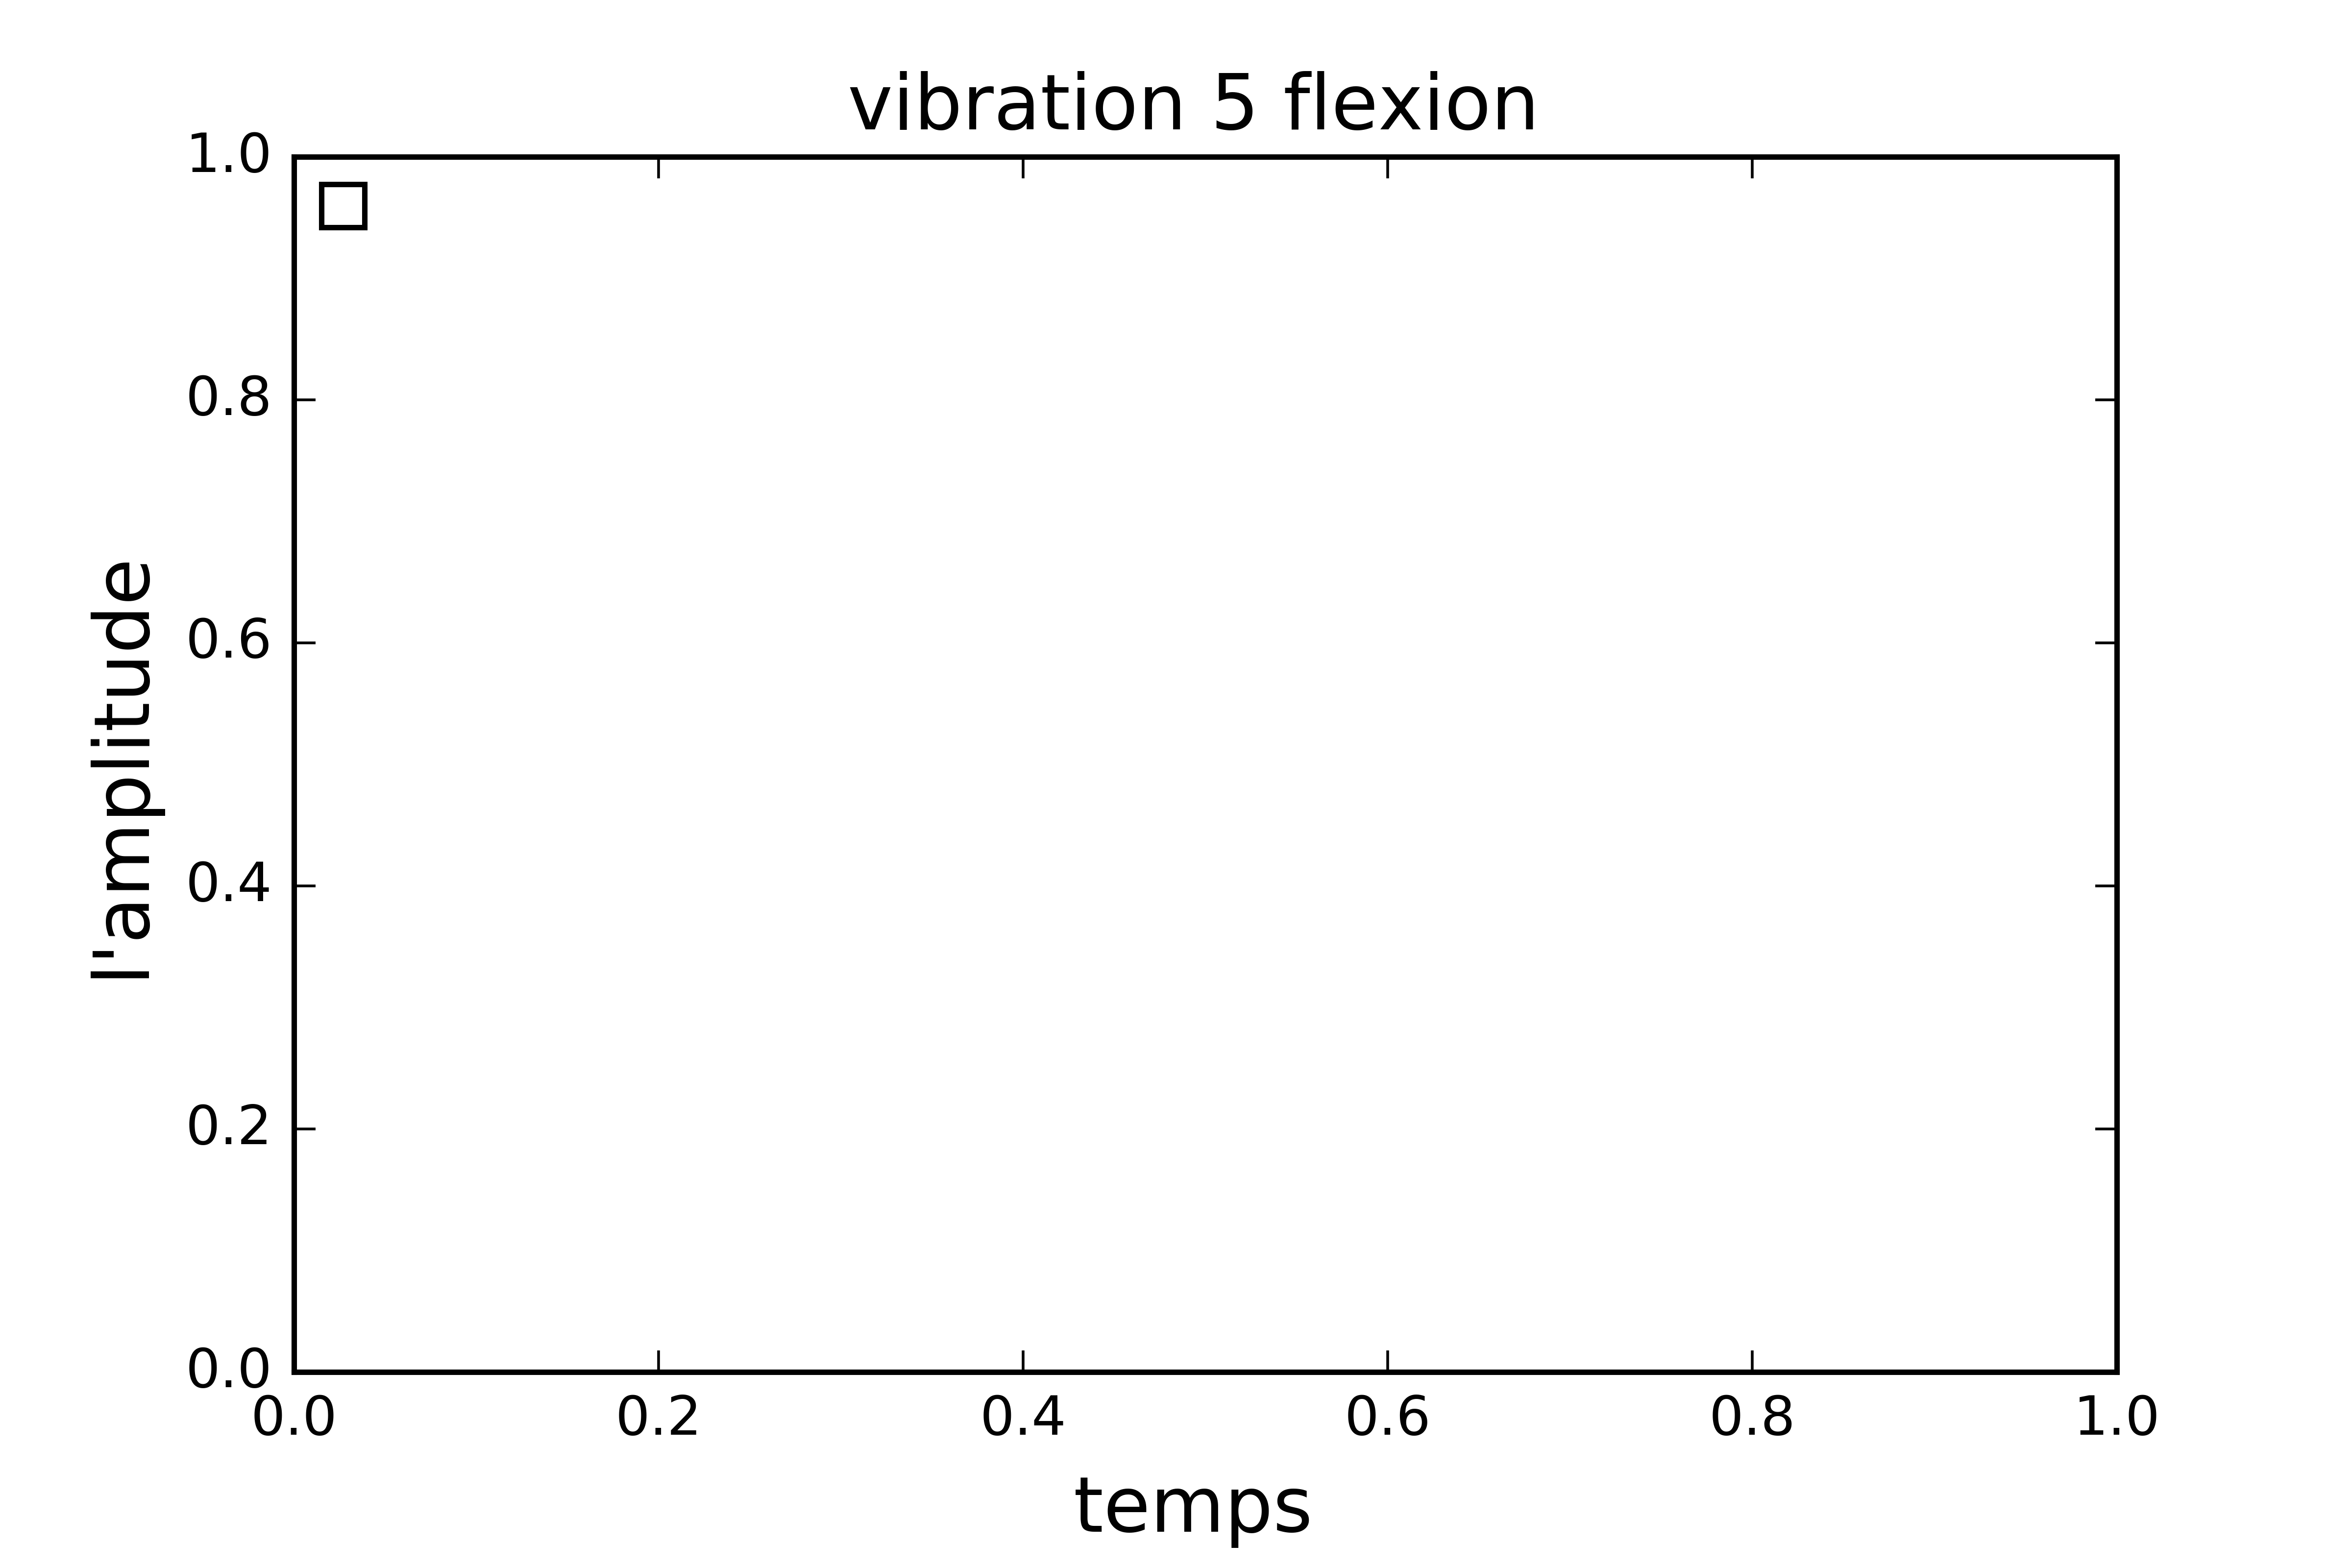
\includegraphics[width=1.0\textwidth]{modee5vt}
\label{figure10}
\caption{vibration5 du temps}
\end{figure}
%%%%%%%%%%%%%%%%%%%%%%%%%%%%%%%%%%%%%%%%%%%%%%%%%%%%%%%%%%%%%%%%%
\chapter{Conclution}

Dans ce 


%%%%%%%%%%%%%%%%%%%%%%%%%%%%%%%%%%%%%%%%%%%%%%%%%%%%%%%%%%%%
%\bibliographystyle{unsrtnat}
%\bibliography{DM-math}
	

\appendix 
\chapter{Code Python}
\section{Listes des fonctions}


\begin{python}
##  trouver les valeurs de gamma
x=np.linspace(0,13*np.pi/4,num=100)
plt.ylim(-1,2) 
plt.plot(x,np.tan(x))
plt.plot(x,np.tanh(x))
plt.xlabel('x', fontsize=14)      
plt.ylabel("deux fonctions", fontsize=14)
plt.title("les points pour tanh(x)=tan(x)", fontsize=14)
plt.legend(['tan(x)','tanh(x)'],loc='lower right', fontsize = 10)
plt.savefig('D:\Tous Les TP\DM-math\ figuretanh.png',dpi=800)



#   definir r_k , k= 1, 2 ,3, 4, 5, 6 ,....
def r_k(n):
    A=np.linspace(1,n,n)
    for i in range(1,n+1):
        A[i-1]=np.pi*(4*i+1)/4
    return A
    while i<N:
        S=section(L,N,i,S0,SL)
        A[i,i]=A[i,i]+(E*S)/h
        A[i,i+1]=-(E*S)/h
        A[i+1,i]=-(E*S)/h
        A[i+1,i+1]=(E*S)/h
        i=i+1
    return A


#   def phi_k pla variation en fonction de x 
def phi_k(r,L):
    y=np.sinh(r*x/L)-np.tanh(r)*np.cosh(r*x/L)-np.sin(r*x/L)+np.tanh(r)*np.cos(r*x/L)
    return y
    
    
#  somme de  phi(x) sans l'implitude 
def somme_phi_k(n,L):
    y=0
    for i in r_k(n):
        y=y+phi_k(i,L)
        i=i+1
    return y
    

# deffinir v_k    
def V_k(n,v0,L):
    A=np.linspace(0,n-1,n)
    i=0
    for r in r_k(n):
        A[i]=(np.cos(r)+np.cosh(r)+np.tanh(r)*(np.sin(r)-np.sinh(r))-2)/r
        i=i+1
    return A
    
    

# definie omega
def omega_k(n,L,E,I,rho,S):
    A=np.linspace(0,n-1,n)
    i=0
    for r in r_k(n):
        A[i]=(r*r)/(L*L)*np.sqrt(E*I/(rho*S))
        i=i+1
    return A
    

#  definir les modes
def mode(n,t,v0,L,E,I,rho,S):
    i=0
    for r in r_k(n):
        y=V_k(n,v0,L)[i]*phi_k(r,L)*np.cos(omega_k(n,L,E,I,rho,S)[i]*t)
        i=i+1
    return y
    
    

#defnir u_k sans somme
def u_k(n,t,v0,L,E,I,rho,S):
    i=0
    for r in r_k(n):
        y=V_k(n,v0,L)[i]*phi_k(r,L)*np.cos(omega_k(n,L,E,I,rho,S)[i]*t)
        i=i+1
    return y
    
    

\end{python}

\subsection{Paramètres du problème}

\begin{python}
#Paramettre du probleme:
S0=16.2
SL=6.7
L=51.5
err=0.076
rho=1600
E=21300*10**6
omega=2*np.pi
N=5 # Premiere etude avec N=5
\end{python}

\section{Étude pour N=5}
\subsection{Solution approchée pour N=5}
\begin{python}
A=matrixA(E,L,N,S0,SL)
B=vecteurB(rho,omega,N,S0,SL)
#Condition limite:
A[0,0]=1
A[0,1]=0
B[0]=0
uh=np.linalg.solve(A,B) #Resolution du syteme : solution approchee pour N=5

x=np.linspace(0,L,100) #Axe horizontale pour la solution analytique
r=np.linspace(0,L,N+1) #Array avec tout les noeuds en fonction de N
u5=u2(E,L,rho,omega,N,S0,SL,x)

p1=plt.plot(r,uh,marker='o',label='Solution Approchee Uh')
plt.plot(x,u2(E,L,rho,omega,N,S0,SL,x),'r',label='Solution Analytique U')
plt.legend(loc='lower right')
plt.xlabel('r',fontsize=12)
plt.ylabel('U & Uh',fontsize=12)
plt.title("Solutions Approchees & Analytique pour N="+str(N), fontsize=14)
plt.savefig('D:\Google Drive - Mohamed\Cours\S1\Element Fini\TP 1\U Uh N5.png',dpi=800)
\end{python}
\subsection{Erreur relative pour N=5}
\begin{python}
ur=u2(E,L,rho,omega,N,S0,SL,r) #On calcul les valeurs theoriques pour differents noeuds (array "r")
error=np.absolute(ur-uh)/ur #formule pour chaque point

plt.plot(r,error*100,marker='o') #pourcentage
#plt.axhline(y=err*100, hold=None)
plt.ylabel('$\epsilon$ : erreur relative en $\%$',fontsize=12)
plt.xlabel('$h$',fontsize=12)
plt.title("Erreur relative a differents noeuds pour N="+str(N), fontsize=14)
plt.savefig('D:\Google Drive - Mohamed\Cours\S1\Element Fini\TP 1\Erreur relative N5.png',dpi=800) 
\end{python}
\section{Étude pour différents N}
\subsection{Solutions Approchées pour différents N}
\begin{python}
#Paramettre du probleme:
S0=16.2
SL=6.7
L=51.5
err=0.076
rho=1600
E=21300*10**6
omega=2*np.pi
Nmin=4 #nombre de noeud minimal
Nmax=20 #nombre de noeud maximal

for i in range (Nmin,Nmax+1,4):
    N=i
    x=np.linspace(0,L,100)
    r=np.linspace(0,L,N+1)
    A=matrixA(E,L,N,S0,SL)
    B=vecteurB(rho,omega,N,S0,SL)
    #Condition limite:
    A[0,0]=1
    A[0,1]=0
    B[0]=0
    uh=np.linalg.solve(A,B)
    plt.plot(r,uh,label='N='+str(N),)
plt.plot(x,u2(E,L,rho,omega,N,S0,SL,x),'k',label='Solution Analytique')
plt.legend(loc='lower right')
plt.xlabel('$r$',fontsize=12)
plt.ylabel('$u_{i}$',fontsize=12)
plt.title("Solutions Approchees & Analytique", fontsize=14)
plt.savefig('D:\Google Drive - Mohamed\Cours\S1\Element Fini\TP 1\Solutions Approchees & Analytique.png',dpi=800)
\end{python}
\subsection{Erreur relative en fonction de h}

\begin{python}
error=np.zeros(Nmax)
H=np.zeros(Nmax)
for i in range (Nmin,Nmax):
    N=i
    h=L/N
    x=np.linspace(0,L,100)
    r=np.linspace(0,L,N+1)
    A=matrixA(E,L,N,S0,SL)
    B=vecteurB(rho,omega,N,S0,SL)
    #Condition limite:
    A[0,0]=1
    A[0,1]=0
    B[0]=0
    uh=np.linalg.solve(A,B)
    U=u2(E,L,rho,omega,N,S0,SL,r)
    error[i-Nmin]=(np.absolute(U[N]-uh[N])/U[N])
    H[i-Nmin]=h
plt.plot(H,error,label='$Err(h)$')
#plt.axhline(y=err, hold=None) #tracer ligne pour errmax
plt.ylabel('$\epsilon$ : erreur relative en $\%$ en fonction de N',fontsize=12)
plt.xlabel('h',fontsize=12)
plt.title("Erreur relative au noeud $r_{n}=L$", fontsize=14)
plt.savefig('D:\Google Drive - Mohamed\Cours\S1\Element Fini\TP 1\Erreur relative fct de h.png',dpi=800) 
\end{python}
\subsection{Erreur relative en fonction de N}

\begin{python}
plt.plot(L/H,error*100,label='$Err(N)$')
plt.ylabel('$\epsilon$ : erreur relative en $\%$ en fonction de N',fontsize=12)
plt.xlabel('N',fontsize=12)
plt.title("Erreur relative au noeud $r_{n}=L$", fontsize=14)
plt.savefig('D:\Google Drive - Mohamed\Cours\S1\Element Fini\TP 1\Erreur relative fct de N.png',dpi=800)
\end{python}

\section{Étude de l'erreur relative en fonction du polynôme interpolation}
\begin{python}
\end{python}


\end{document}
\grid
